%==================================================================================================
\section{Exemplos de Verificação} \label{ExemplosMT}
%==================================================================================================

\textcolor{red}{REVISAR}

Para verificação das formulações implementadas, realizaram-se algumas simulações de problemas bidimensionais bastante conhecidos. Utilizando-se o problema de escoamento em uma cavidade, proposto por \citeonline{ghia1982high}, foi possível observar-se os impactos na solução com o uso de diferentes elementos, seguido de uma análise da convergência para tais elementos, e, por fim, uma verificação dos efeitos da inclusão de modelos de turbulência frente a uma simulação direta. Para a verificação prévia das implementações tridimensionais, adotando-se a geometria de uma cavidade tridimensional, simulou-se o problema \textit{Taylor-Green Vortex} (TGV) \cite{shapiro1993use}. Por fim, simulou-se o escoamento sobre um cilindro proposto por \citeonline{tezduyar1992incompressible,codina2006numerical,najafi2012meshless,fernandes2020tecnica}, analisando-se o comportamento transiente dos coeficientes de arrasto e de sustentação para diferentes modelos e aproximações. Os resultados obtidos para cada uma das simulações são apresentados nos Apêndices \ref{Ap:Cavity} ao \ref{Ap:cylinder}.

%==================================================================================================
\subsection{Cavidade bidimensional}
%==================================================================================================

Um problema comumente utilizado na literatura como \textit{benchmark}, trata-se de uma cavidade quadrada ($\Omega=[-1,1]^2$) com paredes aderentes, onde o fluido encontra-se confinado e sujeito a uma velocidade prescrita $\BB{u}_\infty$ ocasionada devido ao deslizamento de uma parede na face superior da cavidade. Assim são observados os efeitos provocados no escoamento devido à diferentes números de Reynolds, o qual é calculado por meio da equação \eqref{eq:Reynolds}:

\begin{equation}
    \Rey=\frac{\rho L\norm{\BB{u}_\infty}}{\mu}\text{,}
    \label{eq:Reynolds}
\end{equation}

\noindent em que $L$ é o comprimento característico, que no caso analisado é igual ao lado da cavidade. Dessa forma considera-se uma velocidade constante para todas as análises de $\BB{u}_\infty=(1,0)\trans$, sendo os diferentes números de Reynolds obtidos pela variação da viscosidade do fluido. A Figura \ref{fig:cavity} apresenta esquematicamente o problema simulado.

\begin{figure}[h!]
    \centering
    \caption{Cavidade bidimensional - Desenho esquemático}
    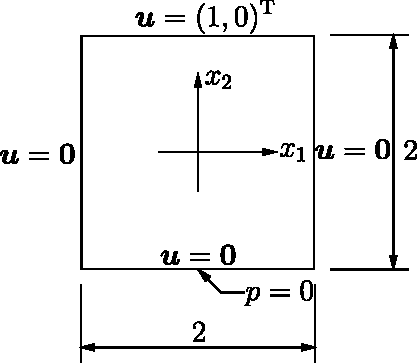
\includegraphics[width=.4\linewidth]{Figuras/Cavity/cavidade.pdf}
    \\Fonte: Autoria Própria (\the\year).
    \label{fig:cavity}
\end{figure}

Pelo fato de o problema possuir apenas fronteiras de Dirichlet, o condicionamento da solução do campo de pressões é garantido pela aplicação de uma condição de pressão nula no centro da aresta inferior da cavidade, conforme visto na figura acima. Também se observa que existe uma descontinuidade nas condições de contorno no encontro entre as paredes da cavidade e seu topo, podendo ser consideradas velocidades nulas ou igual à velocidade do topo. No problema em questão considerou-se que a velocidade nesse ponto é igual à $\BB{u}_\infty$.

A simulação foi conduzida considerando malhas estruturadas com orientação à esquerda para elementos triangulares. Assim observou-se a solução obtida para três casos: elementos de aproximação linear (estabilizado por SUPG/PSPG), quadrática (estabilizado por SUPG/PSPG e VMS) e P2P1 sem termos estabilizadores, sendo todos simulados tanto em DNS e com aplicação do modelo LES. A Tabela \ref{tab:cavity-mesh} apresenta as características das malhas utilizadas, sendo $n_u$ e $n_p$ o número de nós para interpolação do campo de velocidades e de pressões, respectivamente. A Figura \ref{fig:cavity-mesh} apresenta as malhas utilizadas para a simulação.

\begin{table}[h!]
    \centering
    \caption{Cavidade bidimensional - Características das malhas utilizadas.}
    \begin{tabular}{lcccc}
        \hline
        Malha      & Elementos & $n_u$ & $n_p$ & DOF   \\\hline
        Linear     & 12800     & 6561  & 6561  & 19683 \\
        Quadrático & 3200      & 6561  & 6561  & 19683 \\
        P2P1       & 3200      & 6561  & 1681  & 14803 \\\hline
    \end{tabular}
    \\Fonte: Autoria Própria (\the\year).
    \label{tab:cavity-mesh}
\end{table}

\begin{figure}[h!]
    \centering
    \caption{Cavidade bidimensional - Malhas utilizadas.}
    \begin{subfigure}{0.49\textwidth}
        \centering
        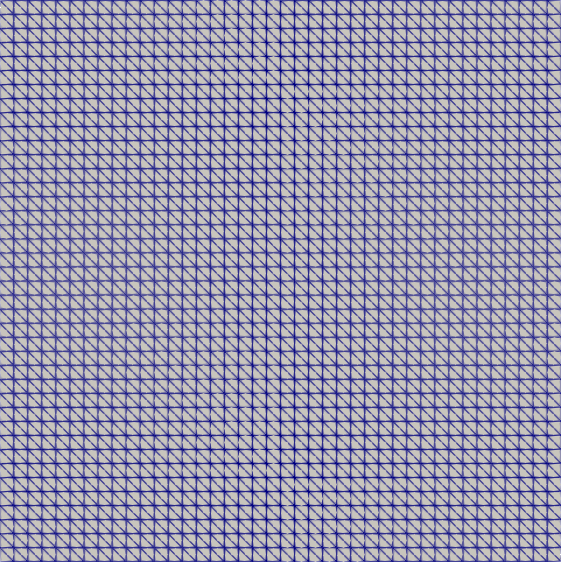
\includegraphics[width=.8\linewidth]{Figuras/Cavity/m1.png}
        \caption{Malha de elementos quadráticos e P2P1.}
    \end{subfigure}
    \begin{subfigure}{0.49\textwidth}
        \centering
        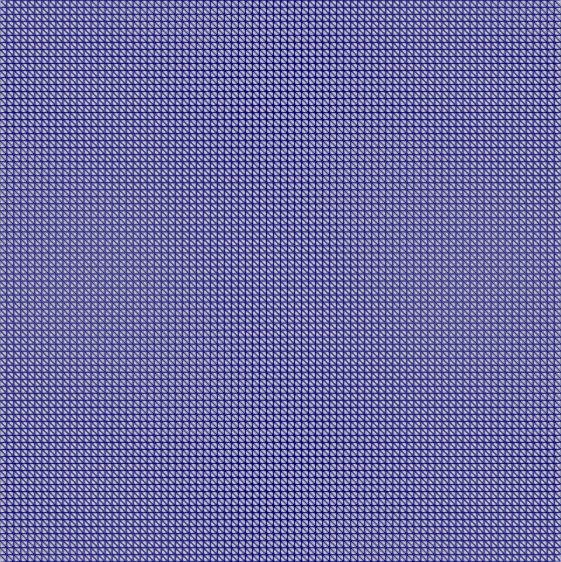
\includegraphics[width=.8\linewidth]{Figuras/Cavity/m1-Lin.png}
        \caption{Malha de elementos lineares.}
    \end{subfigure}
    \\Fonte: Autoria Própria (\the\year).
    \label{fig:cavity-mesh}
\end{figure}

O fluido possui massa específica $\rho=1$ para todas as análises e viscosidade dinâmica variando de forma a se obter diferentes números de Reynolds. Assim os valores da viscosidade serão de $\mu=0,02$, $\mu=5\times10^{-3}$, $\mu=2\times10^{-3}$, $\mu=4\times10^{-4}$, $\mu=2,6667\times10^{-4}$ e $\mu=2\times10^{-4}$, resultando em $\Rey=100$, $\Rey=400$, $\Rey=1000$, $\Rey=5000$, $\Rey=7500$ e $\Rey=10000$, respectivamente. O problema parte do repouso em todas as simulações, o passo de tempo foi de $\Delta t=0,1$ e a simulação foi mantida até que a estacionariedade do fluxo fosse alcançada, sendo o esquema de integração temporal obtido a partir de $\rho_\infty=0,0$. O valor da constante de Smagorinsky foi de $C_S=0,10$.

Os resultados obtidos foram comparados com aqueles apresentados por \citeonline{ghia1982high}. A Figura \ref{fig:cavity-results} apresenta os valores do campo de velocidades sobre as linhas médias da cavidade ($x_1=0$ e $x_2=0$).

\begin{figure}[h!]
    \centering
    \caption{Cavidade bidimensional - Valores do campo de velocidades sobre as linhas médias.}
    \begin{subfigure}{0.4\textwidth}
        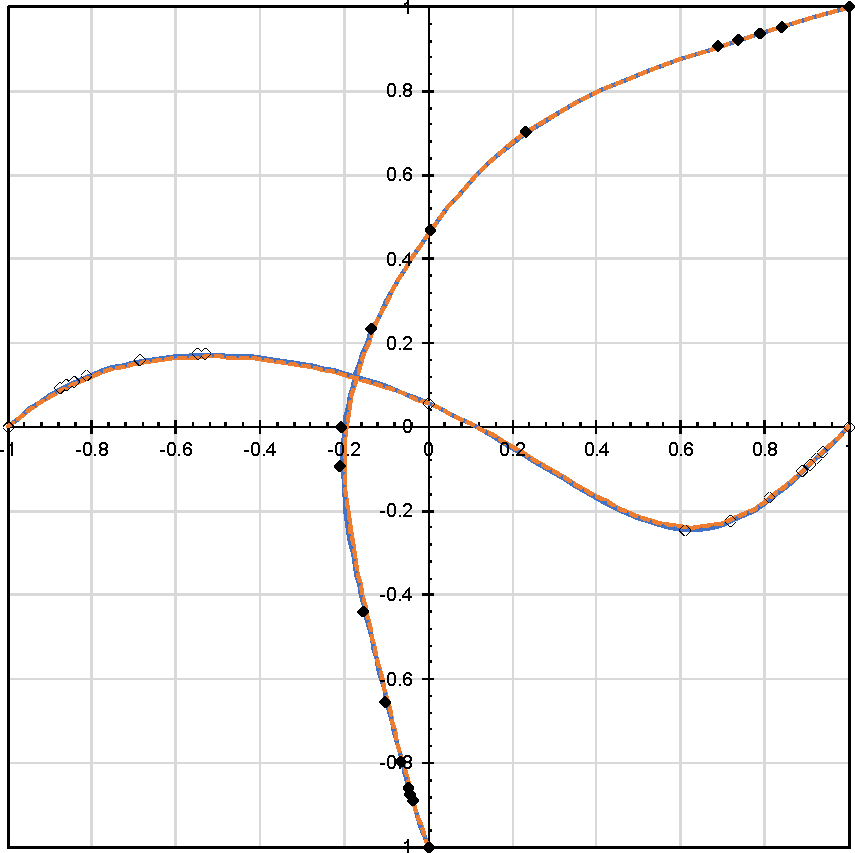
\includegraphics[width=\linewidth]{Figuras/Cavity/Re100.pdf}
        \caption{$\Rey=100$}
    \end{subfigure}
    \begin{subfigure}{0.4\textwidth}
        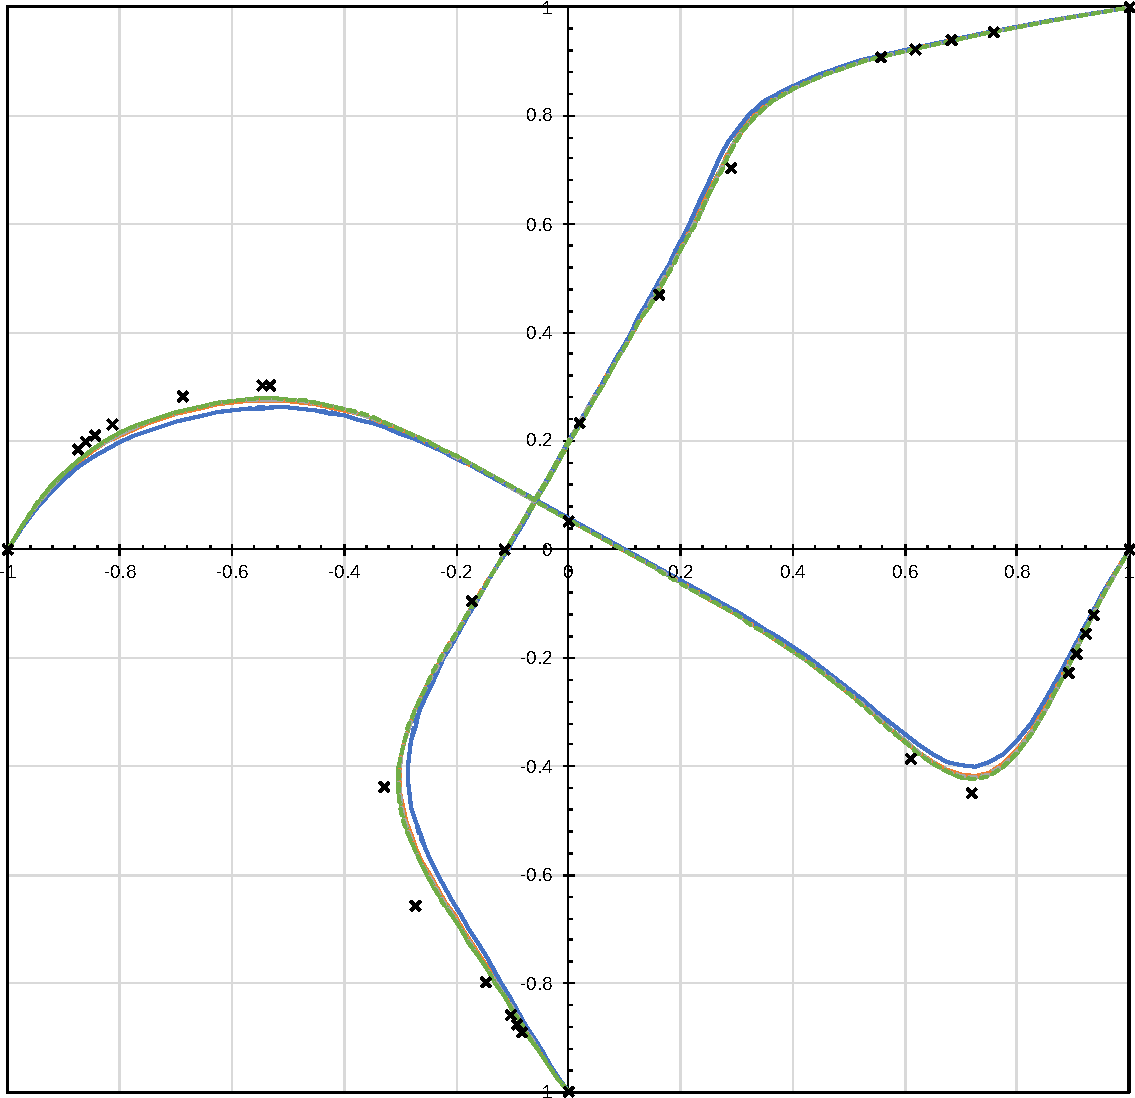
\includegraphics[width=\linewidth]{Figuras/Cavity/Re400.pdf}
        \caption{$\Rey=400$}
    \end{subfigure}
    \begin{subfigure}{0.4\textwidth}
        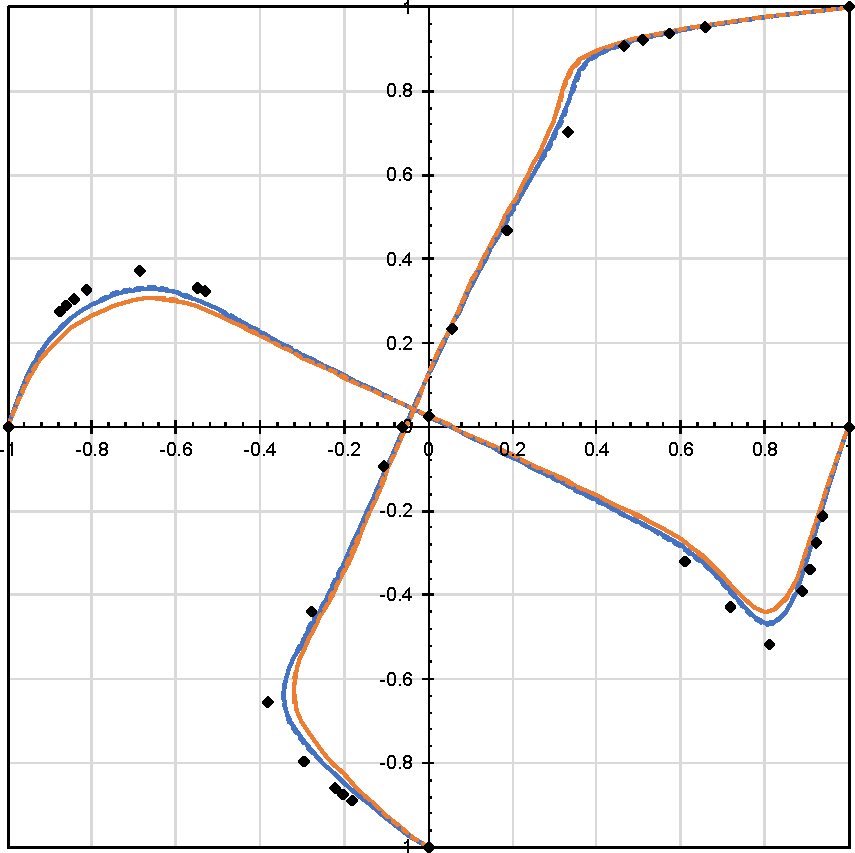
\includegraphics[width=\linewidth]{Figuras/Cavity/Re1000.pdf}
        \caption{$\Rey=1000$}
    \end{subfigure}
    \begin{subfigure}{0.4\textwidth}
        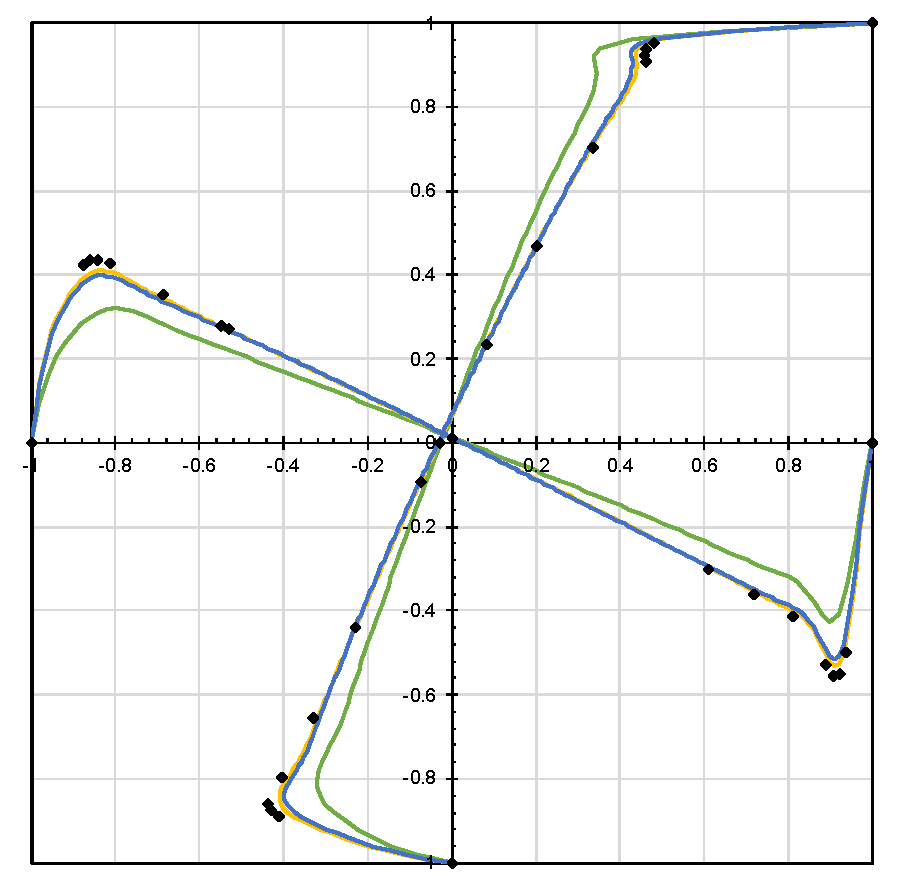
\includegraphics[width=\linewidth]{Figuras/Cavity/Re5000.pdf}
        \caption{$\Rey=5000$}
    \end{subfigure}
    \begin{subfigure}{0.4\textwidth}
        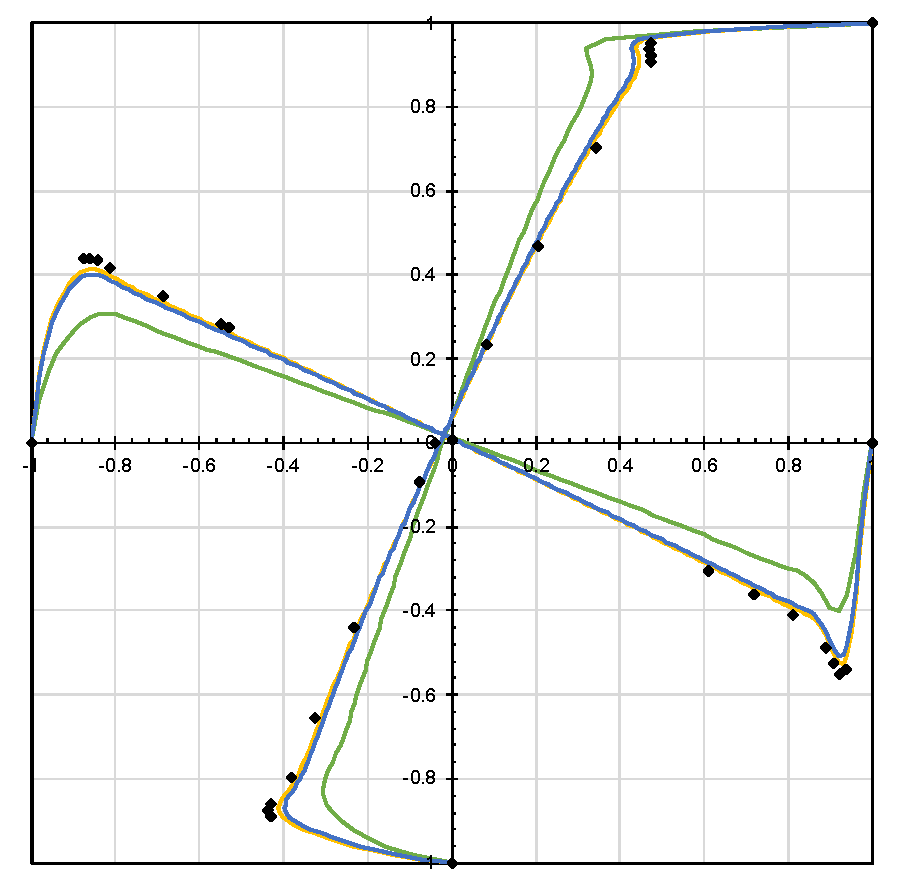
\includegraphics[width=\linewidth]{Figuras/Cavity/Re7500.pdf}
        \caption{$\Rey=7500$}
    \end{subfigure}
    \begin{subfigure}{0.4\textwidth}
        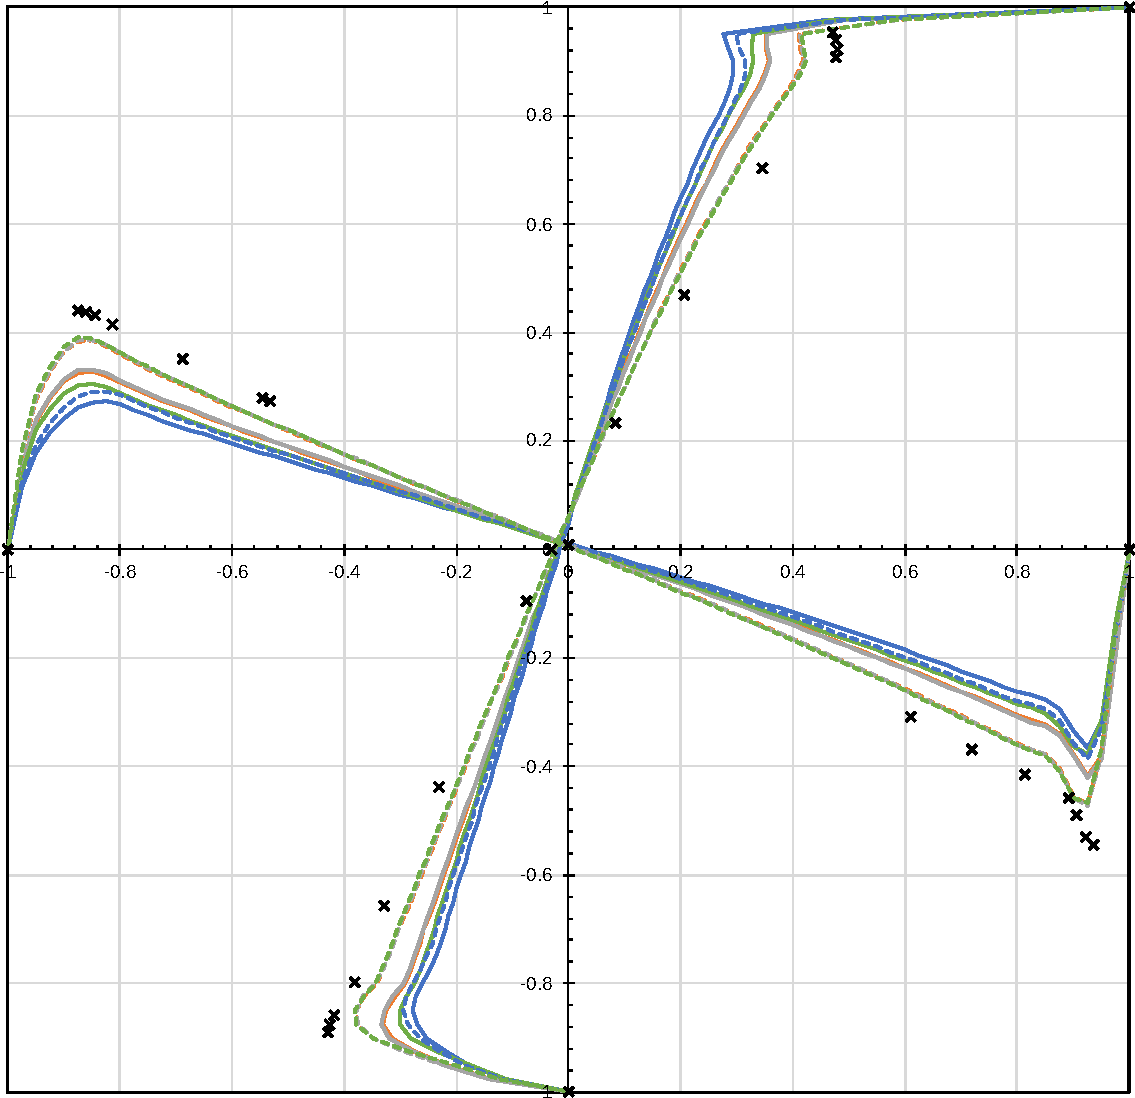
\includegraphics[width=\linewidth]{Figuras/Cavity/Re10000.pdf}
        \caption{$\Rey=10000$}
    \end{subfigure}
    \begin{subfigure}{\textwidth}
        \centering
        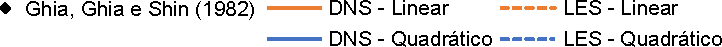
\includegraphics[width=.7\linewidth]{Figuras/Cavity/legenda.pdf}
    \end{subfigure}
    \\Fonte: Autoria Própria (\the\year).
    \label{fig:cavity-results}
\end{figure}

A Figura \ref{fig:cavity-results2} apresenta o campo de velocidades na cavidade após o escoamento atingir seu estado estacionário segundo a simulação LES utilizando elementos quadráticos.

\begin{figure}[h!]
    \centering
    \caption{Cavidade bidimensional - Campo de velocidades em regime estacionário.}
    \begin{subfigure}{0.32\textwidth}
        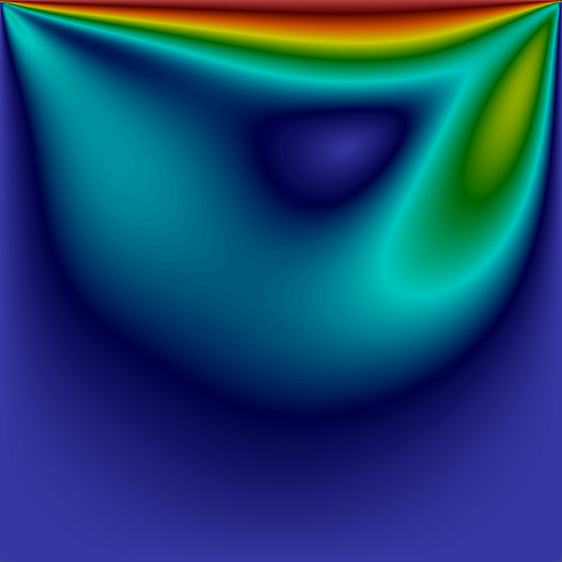
\includegraphics[width=\linewidth]{Figuras/Cavity/Re100.png}
        \caption{$\Rey=100$}
    \end{subfigure}
    \begin{subfigure}{0.32\textwidth}
        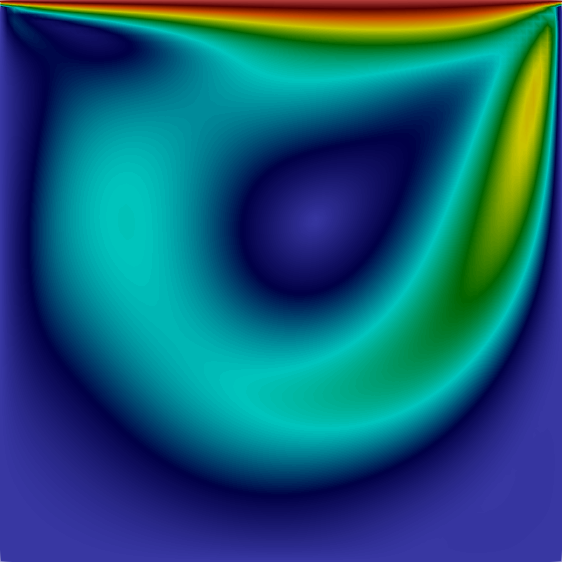
\includegraphics[width=\linewidth]{Figuras/Cavity/Re400.png}
        \caption{$\Rey=400$}
    \end{subfigure}
    \begin{subfigure}{0.32\textwidth}
        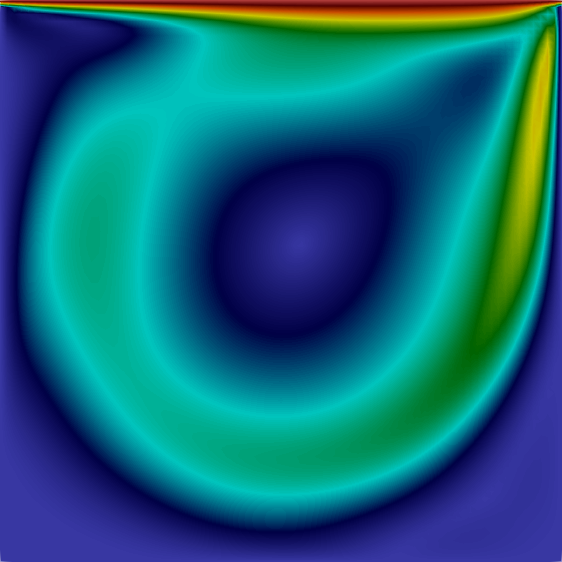
\includegraphics[width=\linewidth]{Figuras/Cavity/Re1000.png}
        \caption{$\Rey=1000$}
    \end{subfigure}
    \begin{subfigure}{0.32\textwidth}
        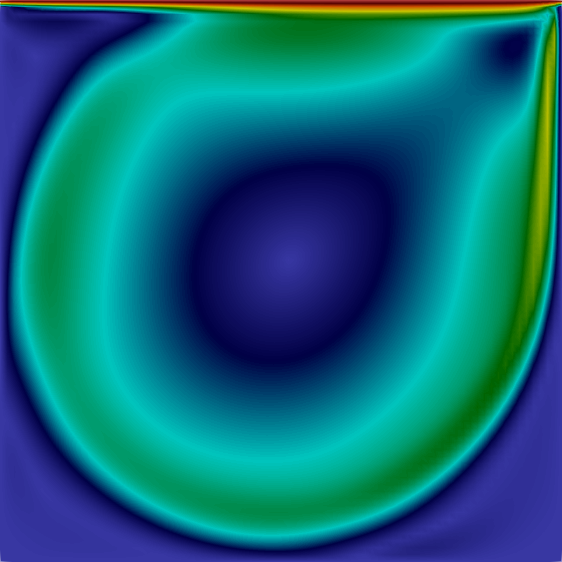
\includegraphics[width=\linewidth]{Figuras/Cavity/Re5000.png}
        \caption{$\Rey=5000$}
    \end{subfigure}
    \begin{subfigure}{0.32\textwidth}
        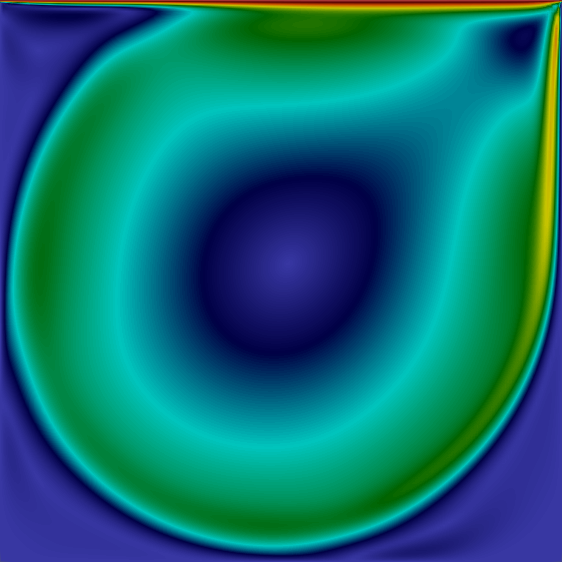
\includegraphics[width=\linewidth]{Figuras/Cavity/Re7500.png}
        \caption{$\Rey=7500$}
    \end{subfigure}
    \begin{subfigure}{0.32\textwidth}
        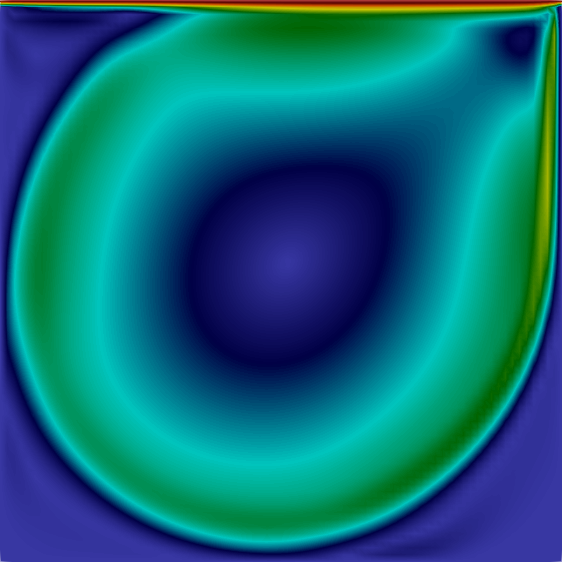
\includegraphics[width=\linewidth]{Figuras/Cavity/Re10000.png}
        \caption{$\Rey=10000$}
    \end{subfigure}
    \begin{subfigure}{0.4\textwidth}
        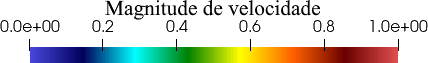
\includegraphics[width=\linewidth]{Figuras/Cavity/legenda.png}
    \end{subfigure}
    \\Fonte: Autoria Própria (\the\year).
    \label{fig:cavity-results2}
\end{figure}

Pelo fato da malha ser grosseira, percebe-se que os resultados divergem ligeiramente do esperado em relação à referência, principalmente para números de Reynolds elevados. No entanto, para esse nível de refinamento é possível observar que os elementos lineares, apesar de possuírem mesmo número de graus de liberdade, apresentaram resultados consideravelmente mais discrepantes que os elementos quadráticos. Isso se deve ao fato de que os elementos lineares não possuem a capacidade de representar adequadamente o campo de velocidades, principalmente nas regiões de maior gradiente, como é o caso das paredes da cavidade. Já, para ambos os elementos, verifica-se que a aplicação do modelo LES sobre o escoamento melhorou a representação do campo de velocidades, principalmente para números de Reynolds elevados, onde o escoamento apresenta maior turbulência. Isso deve-se ao fato do modelo ser capaz de capturar os efeitos turbulentos em escalas menores que os elementos da malha, o que não ocorre na simulação DNS.

Para números de Reynolds elevados, no entanto, a aplicação dos demais termos estabilizadores da formulação VMS não afetou significativamente os resultados, em comparação com a simulação estabilizada por SUPG/PSPG. Outro ponto a ser observado é que a consideração de elementos P2P1 sem nenhuma estabilização ainda foi capaz de apresentar resultados muito semelhantes às demais simulações, em termos do campo de velocidades.

Já com relação ao tempo de processamento, observou-se um tempo médio de 0,2285 segundos por iteração para a simulação de elementos lineares em DNS, enquanto para a simulação de elementos quadráticos o tempo médio foi de 0,2032 segundos por iteração, o que resulta em um tempo 12,466\% maior para a simulação de elementos lineares, o que mostra que mesmo possuindo um tempo de processamento maior, seus resultados são menos precisos que o elemento quadrático. Todavia, para a simulação LES, o tempo médio de processamento foi de 0,2134 segundos por iteração em elementos quadráticos, o que resulta em um tempo 5,028\% maior que a simulação DNS de elementos quadráticos, o que mostra que o modelo LES não possui um impacto significativo no tempo de processamento.

Em seguida realizou-se uma análise da dependência da malha para a simulação de elementos quadráticos e P2P1 (estabilizados com SUPG) com $\Rey=10000$, tanto com em DNS quanto utilizando LES, onde se considerou outras duas discretizações, obtidas a partir da subdivisão das arestas do problema em 20 e 8 partes. A Tabela \ref{tab:cavity-mesh2} apresenta as características das malhas utilizadas. A Figura \ref{fig:cavity-mesh2} apresenta as malhas utilizadas para a simulação.

\begin{table}[h!]
    \centering
    \caption{Cavidade bidimensional - Características das malhas utilizadas para a análise de dependência.}
    \begin{tabular}{lcccccc}
        \hline
        Malha               & Elemento   & Subdivisões         & Elementos            & $n_u$ & $n_p$ & DOF  \\\hline
        \multirow{2}{*}{m1} & Quadrático & \multirow{2}{*}{20} & \multirow{2}{*}{800} & 1681  & 1681  & 5043 \\
                            & P2P1       &                     &                      & 1681  & 441   & 3803 \\\hline
        m2                  & Quadrático & 8                   & 128                  & 289   & 289   & 867  \\\hline
    \end{tabular}
    \\Fonte: Autoria Própria (\the\year).
    \label{tab:cavity-mesh2}
\end{table}

\begin{figure}[h!]
    \centering
    \caption{Cavidade bidimensional - Malhas utilizadas para a análise de convergência.}
    \begin{subfigure}{0.49\textwidth}
        \centering
        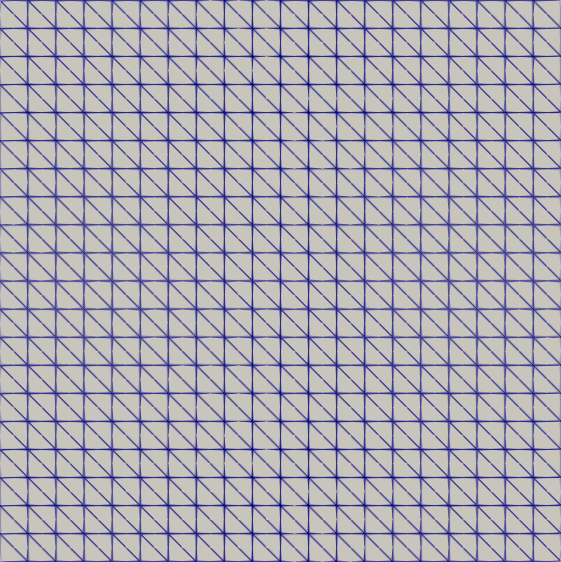
\includegraphics[width=0.8\linewidth]{Figuras/Cavity/m2.png}
        \caption{Malha m1.}
    \end{subfigure}
    \begin{subfigure}{0.49\textwidth}
        \centering
        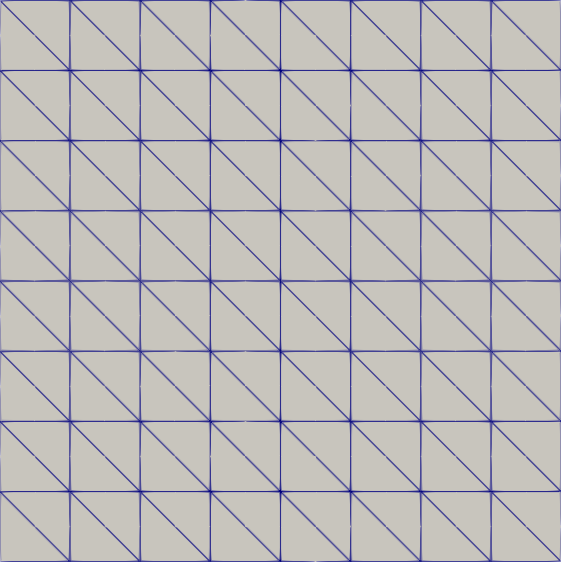
\includegraphics[width=0.8\linewidth]{Figuras/Cavity/m3.png}
        \caption{Malha m2.}
    \end{subfigure}
    \\Fonte: Autoria Própria (\the\year).
    \label{fig:cavity-mesh2}
\end{figure}

Para tais simulações, já se percebeu que o elemento P2P1 divergiu imediatamente na malha m1, mesmo aplicando o modelo LES, o que pode ser explicado pela baixa ordem de aproximação do campo de pressões, que conduz à resultados mais imprecisos conforme a malha se torna mais grosseira. Já na malha m2 se observou que a simulação DNS divergiu para todos os elementos, enquanto o LES se manteve estável durante toda a análise. A Figura \ref{fig:cavity-results3} apresenta os valores do campo de velocidades sobre as linhas médias da cavidade para a malha m1 e m2.

\begin{figure}[h!]
    \centering
    \caption{Cavidade bidimensional - Valores do campo de velocidades sobre as linhas médias para as malhas m1 e m2.}
    \begin{subfigure}{0.49\textwidth}
        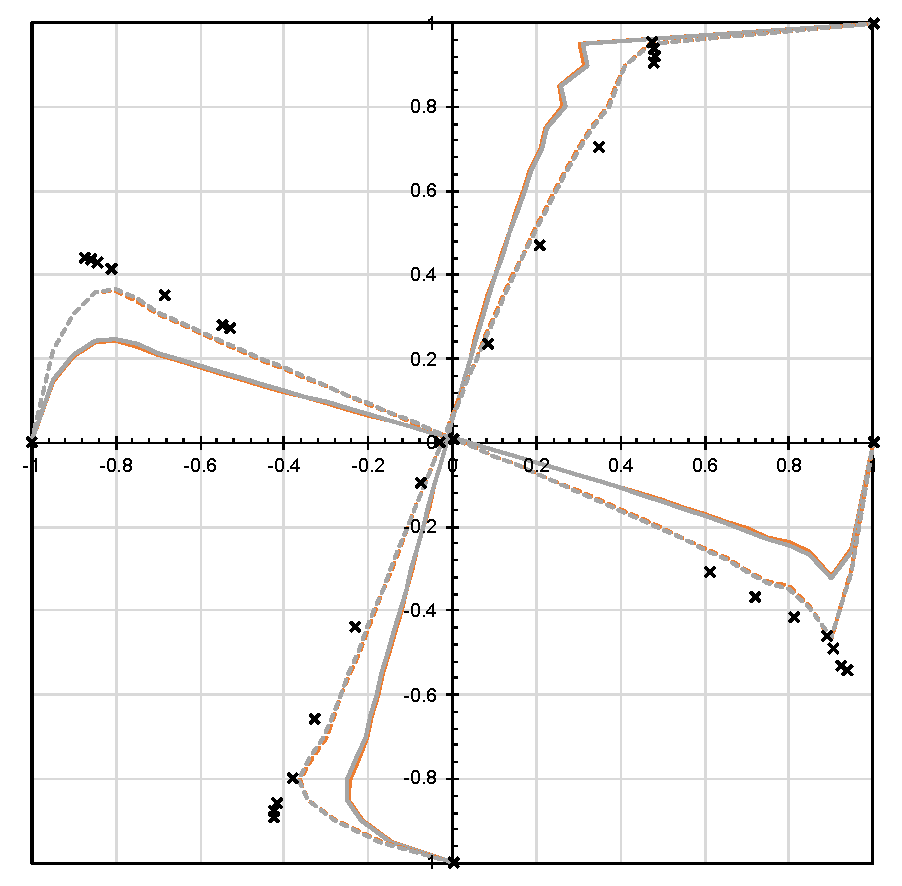
\includegraphics[width=\linewidth]{Figuras/Cavity/res-m1.pdf}
        \caption{Malha m1.}
    \end{subfigure}
    \begin{subfigure}{0.49\textwidth}
        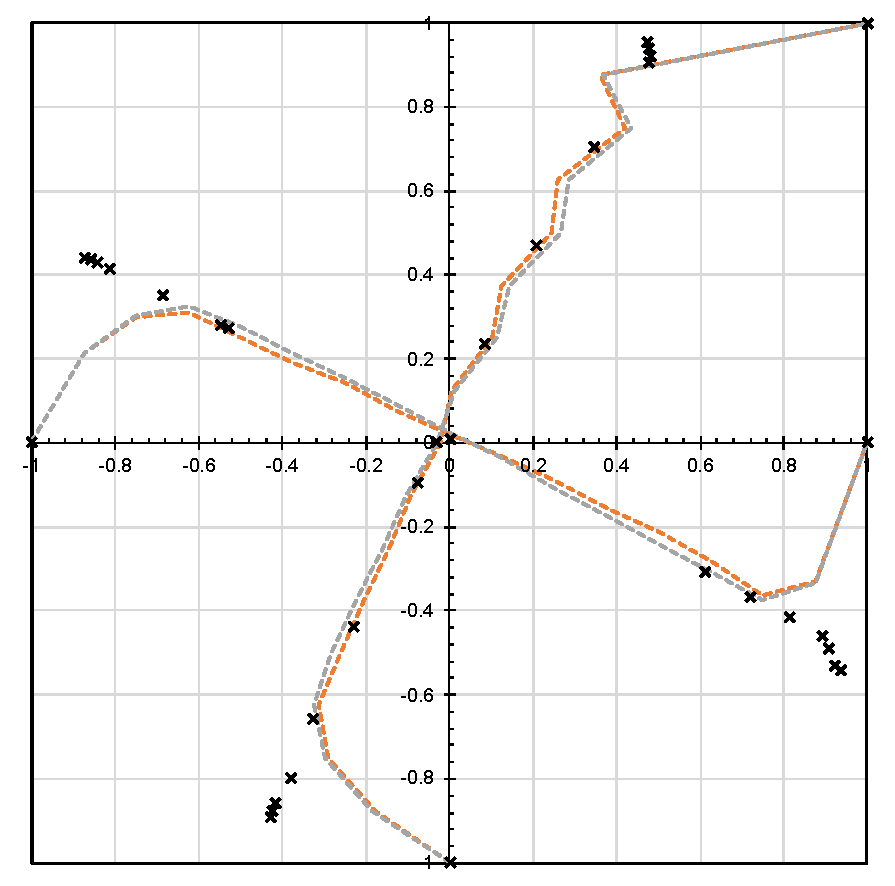
\includegraphics[width=\linewidth]{Figuras/Cavity/res-m2.pdf}
        \caption{Malha m2.}
    \end{subfigure}
    \begin{subfigure}{0.4\textwidth}
        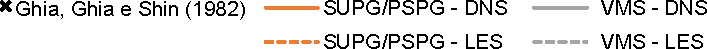
\includegraphics[width=\linewidth]{Figuras/Cavity/legenda-m1m2.pdf}
    \end{subfigure}
    \\Fonte: Autoria Própria (\the\year).
    \label{fig:cavity-results3}
\end{figure}

Sendo assim, constata-se que a aplicação do modelo LES foi capaz de estabilizar a simulação para a malha m2, enquanto para a malha m1, a aplicação do modelo LES foi capaz de estabilizar a simulação apenas para o elemento quadrático. Também se observa que a consideração dos demais termos estabilizadores da formulação VMS melhorou ligeiramente a solução obtida em relação à simulação estabilizada por SUPG/PSPG. A discrepância dos resultados obtidos com relação à referência se deve à baixa qualidade da malha, no entanto é possível observar que a aplicação do modelo LES foi capaz de manter certa representatividade nos resultados.

\begin{comment}
%==================================================================================================
\subsection{\textit{Taylor-Green Vortex} tridimensional}
%==================================================================================================

Para verificação dos modelos implementados em simulações tridimensionais é possível simular o problema de \textit{Taylor-Green Vortex} (TGV), o qual possui solução analítica, dada por \cite{shapiro1993use}:

\begin{subequations}
    \begin{equation}
        \begin{split}
            &\BB{u}_a(\BB{x},t)=\\
            &-\frac{Ae^{-\nu\lambda^2t}}{k^2+l^2}\begin{bmatrix}
                \lambda l\cos{(kx_1)}\sin{(lx_2)}\sin{(mx_3)}+mk\sin{(kx_1)}\cos{(lx_2)}\cos{(mx_3)} \\
                \lambda k\sin{(kx_1)}\cos{(lx_2)}\sin{(mx_3)}-ml\cos{(kx_1)}\sin{(lx_2)}\cos{(mx_3)} \\
                -(k^2+l^2)\cos{(kx_1)}\cos{(lx_2)}\sin{(mx_3)}
            \end{bmatrix}\text{,}
        \end{split}
    \end{equation}
    \begin{equation}
        p_a=p_s-\rho\frac{u_1^2+u_2+u_3^2}{2}\text{.}
    \end{equation}
\end{subequations}

\noindent em que $k$, $l$ e $m$ são constantes arbitrárias, $\lambda^2=k^2+l^2+m^2$, $A$ é a amplitude da componente $u_3$ e $p_s$ é a pressão do ponto de estagnação.

Para o problema numérico foi considerado um cubo ($\Omega=[-1,1]^3$) simulado nos modelos VMS de aproximação linear e quadrática e o LES utilizando elementos Taylor-Hood P2P1. A malha utilizada na discretização conta com 5802 elementos finitos (conforme ilustrado na Figura \ref{fig:TGV-mesh}), sendo 5580 graus de liberdade para VMS linear, 37600 pra VMS quadrático e 29595 para LES.

\begin{figure}[h!]
    \centering
    \caption{Malha utilizada para a simulação de TGV.}
    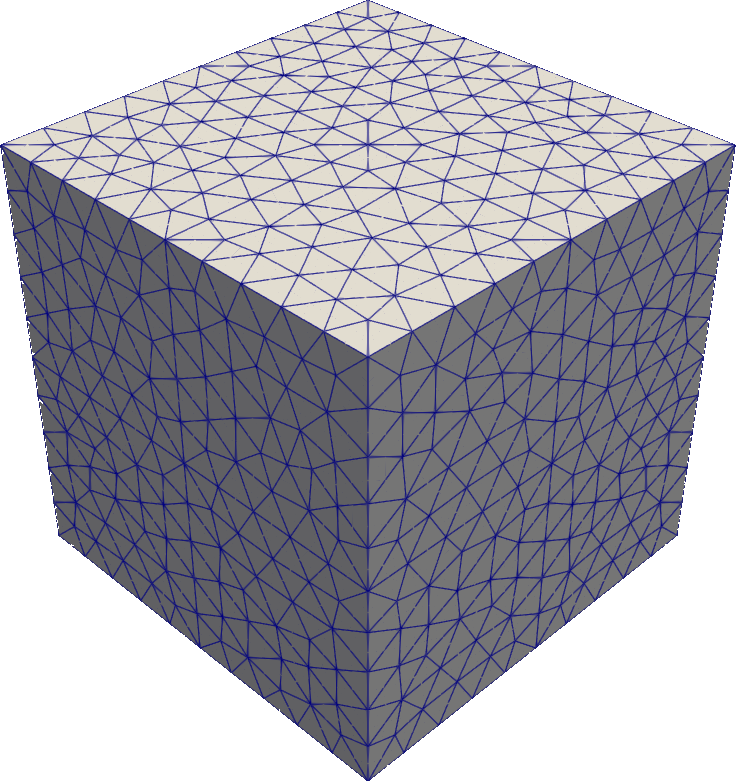
\includegraphics[width=0.4\linewidth]{Figuras/taylor-green/mesh.png}
    \\Fonte: Autoria Própria (\the\year).
    \label{fig:TGV-mesh}
\end{figure}

Como condição inicial impôs-se acelerações, velocidade e pressões iguais à solução analítica com $t=0$ e como condições de contorno aplicou-se velocidades iguais à analítica em toda a fronteira e $p=0$ no centro do domínio. Os valores dos parâmetros foram $k=l=m=\pi$ e $A=\nu=\rho=1$, sendo o período analisado de $t\in[0,0.2]$ com um passo de tempo de $\Delta t=0.001$.

Sendo assim, a Figura \ref{fig:TGV-results} apresenta os valores do campo de velocidades nas linhas $x_2=x_3=0$ ($l1$), $x_1=x_3=0$ ($l2$) e $x_1=x_2=0$ ($l3$) para os instantes $t=0$, $t=0.05$ e $t=0.2$ para todos os modelos considerados.

\begin{figure}[h!]
    \centering
    \caption{Velocidades obtidas na simulação de TGV em:}
    \begin{subfigure}{0.42\textwidth}
        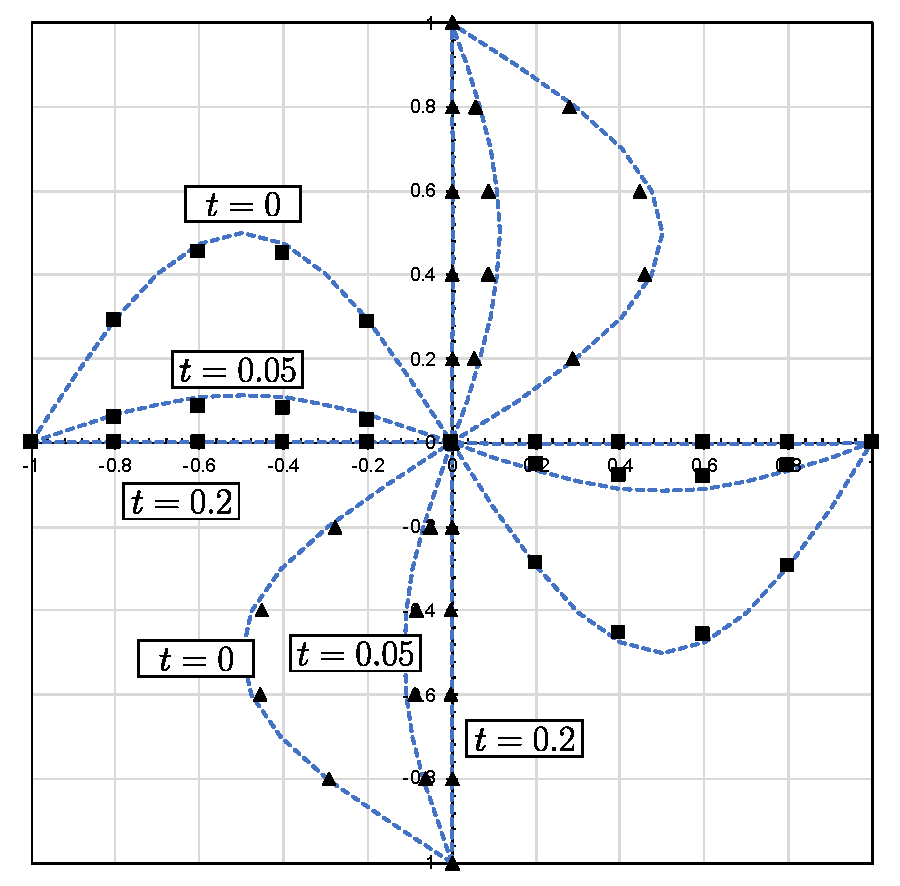
\includegraphics[width=\linewidth]{Figuras/taylor-green/VMS-Lin.pdf}
        \caption{$l1$ e $l2$ para VMS linear.}
    \end{subfigure}
    \begin{subfigure}{0.42\textwidth}
        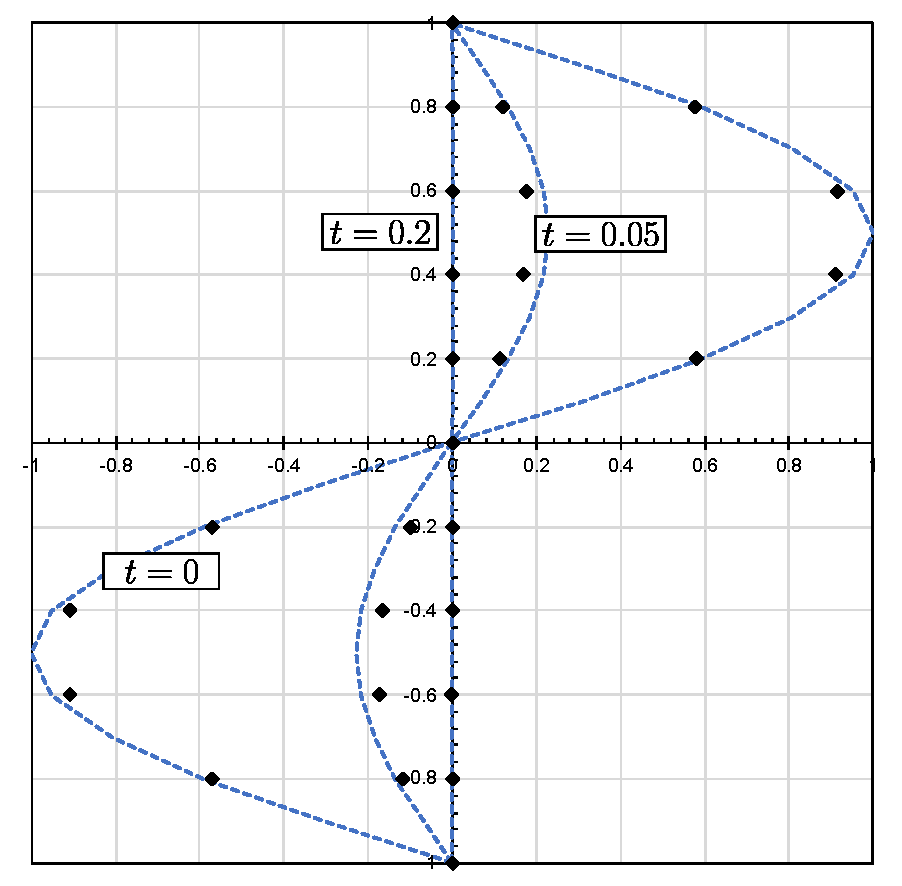
\includegraphics[width=\linewidth]{Figuras/taylor-green/VMS-Lin-uz.pdf}
        \caption{$l3$ para VMS linear.}
    \end{subfigure}
    \begin{subfigure}{0.42\textwidth}
        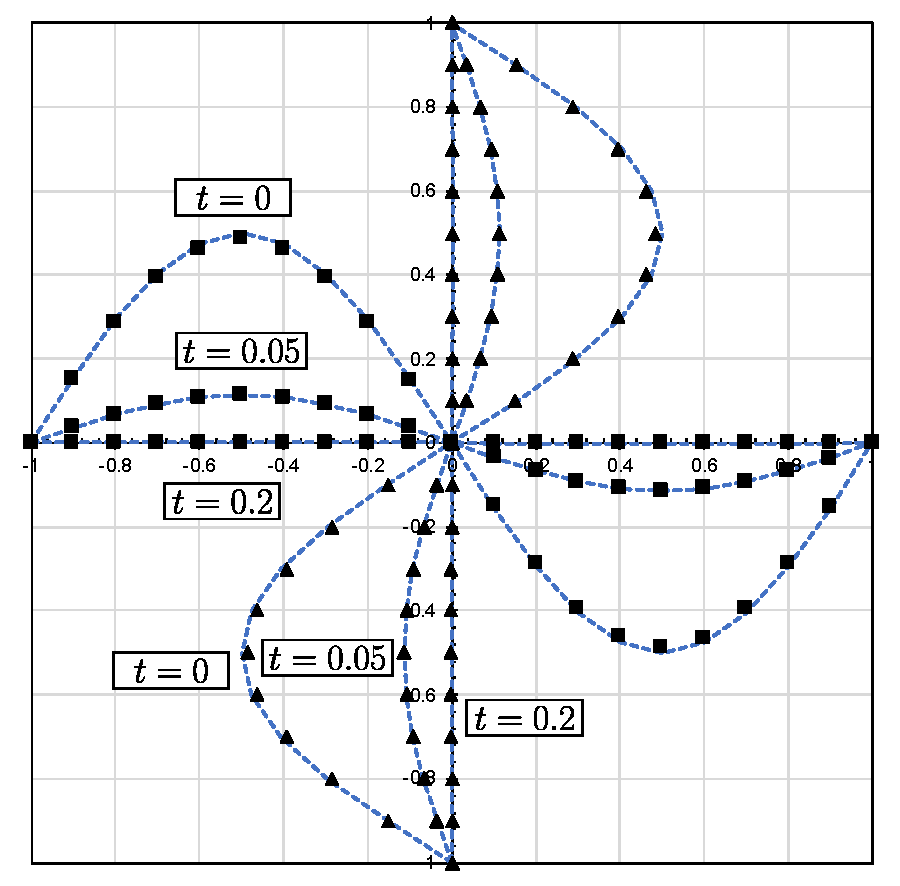
\includegraphics[width=\linewidth]{Figuras/taylor-green/VMS-Qua.pdf}
        \caption{$l1$ e $l2$ para VMS quadrático.}
    \end{subfigure}
    \begin{subfigure}{0.42\textwidth}
        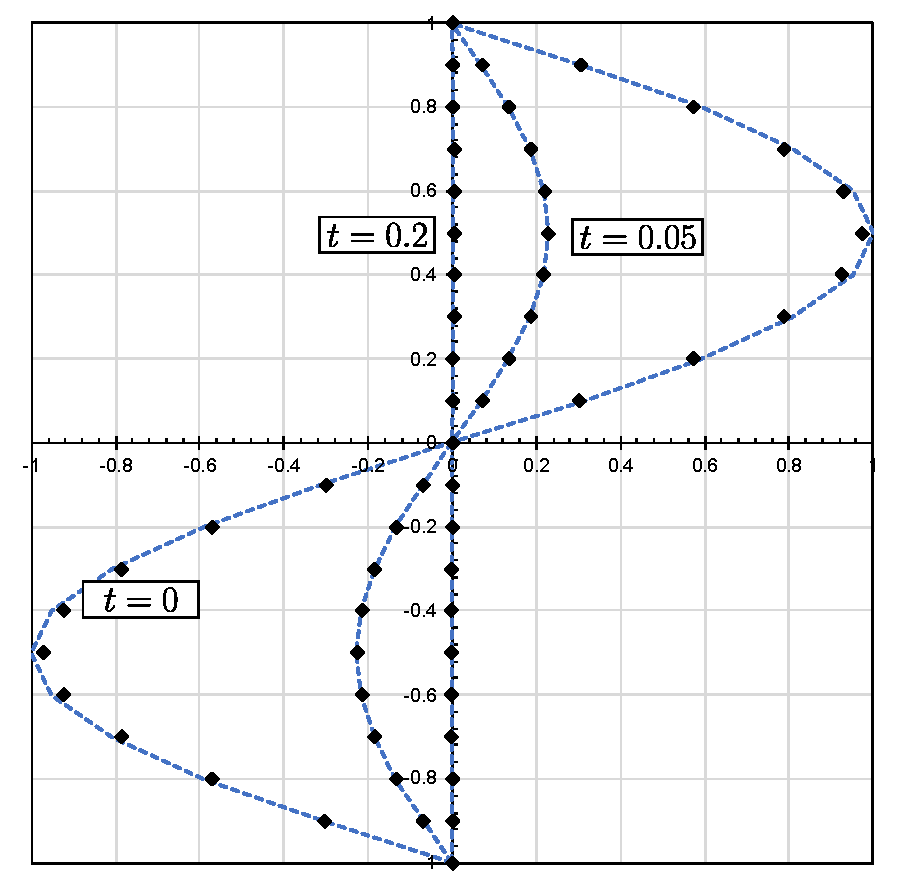
\includegraphics[width=\linewidth]{Figuras/taylor-green/VMS-Qua-uz.pdf}
        \caption{$l3$ para VMS quadrático.}
    \end{subfigure}
    \begin{subfigure}{0.42\textwidth}
        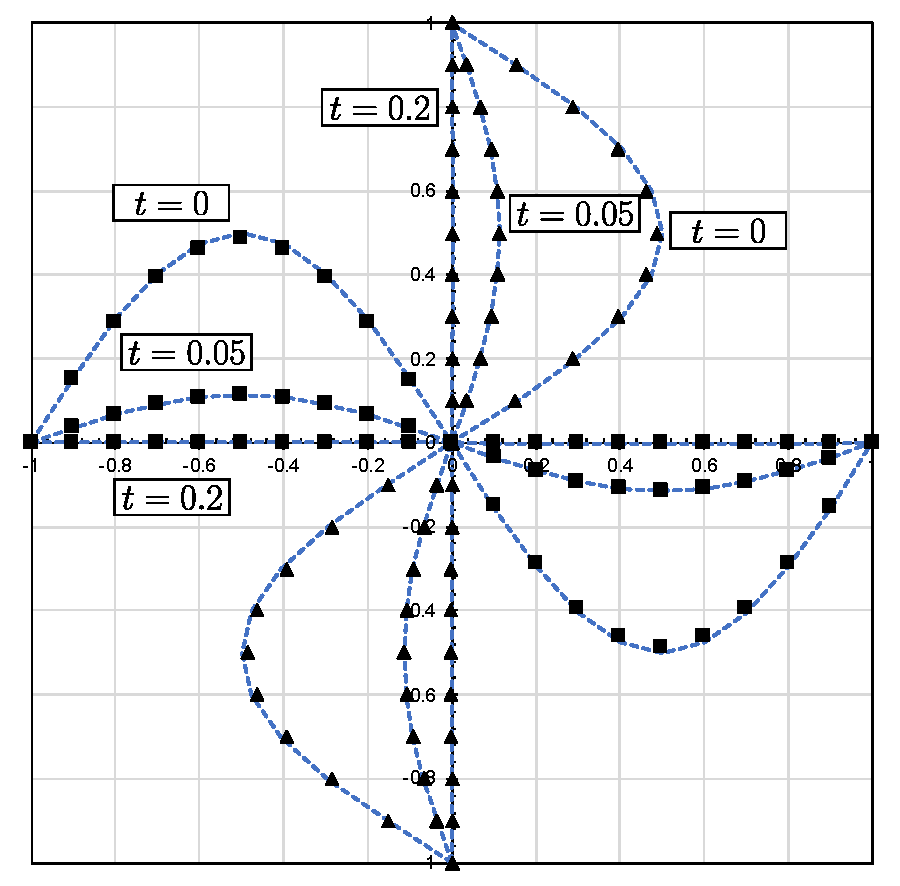
\includegraphics[width=\linewidth]{Figuras/taylor-green/LES.pdf}
        \caption{$l1$ e $l2$ para LES.}
    \end{subfigure}
    \begin{subfigure}{0.42\textwidth}
        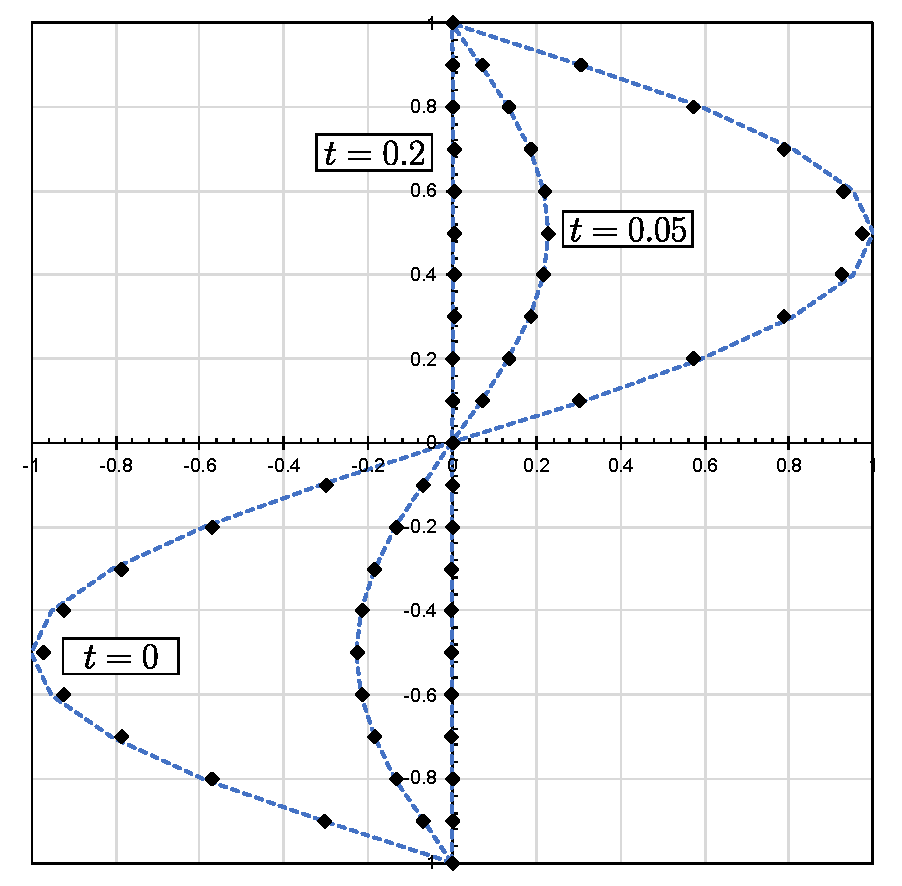
\includegraphics[width=\linewidth]{Figuras/taylor-green/LES-uz.pdf}
        \caption{$l3$ para LES.}
    \end{subfigure}
    \begin{subfigure}{0.42\textwidth}
        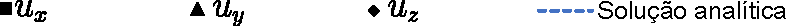
\includegraphics[width=\linewidth]{Figuras/taylor-green/legenda.pdf}
    \end{subfigure}
    \\Fonte: Autoria Própria (\the\year).
    \label{fig:TGV-results}
\end{figure}

Para comparação com a solução analítica, tomou-se a medida do erro em $L^2$, expresso por \cite{dumon2011proper}:

\begin{equation}
    \norm{\BB{e}}=\norm{\BB{u}-\BB{u}_a}_{L^\infty(L^2(\Omega))}=\max_{0<t\leq T}{\left[\int_\Omega{\norm{\BB{u}-\BB{u}_a}^2d\Omega}\right]}\text{,}
\end{equation}

\noindent o qual é representado ao longo do tempo de acordo com a Figura \ref{fig:TGV-L2}:

\begin{figure}[h!]
    \centering
    \caption{Medidas de $L^2$ ao longo do tempo.}
    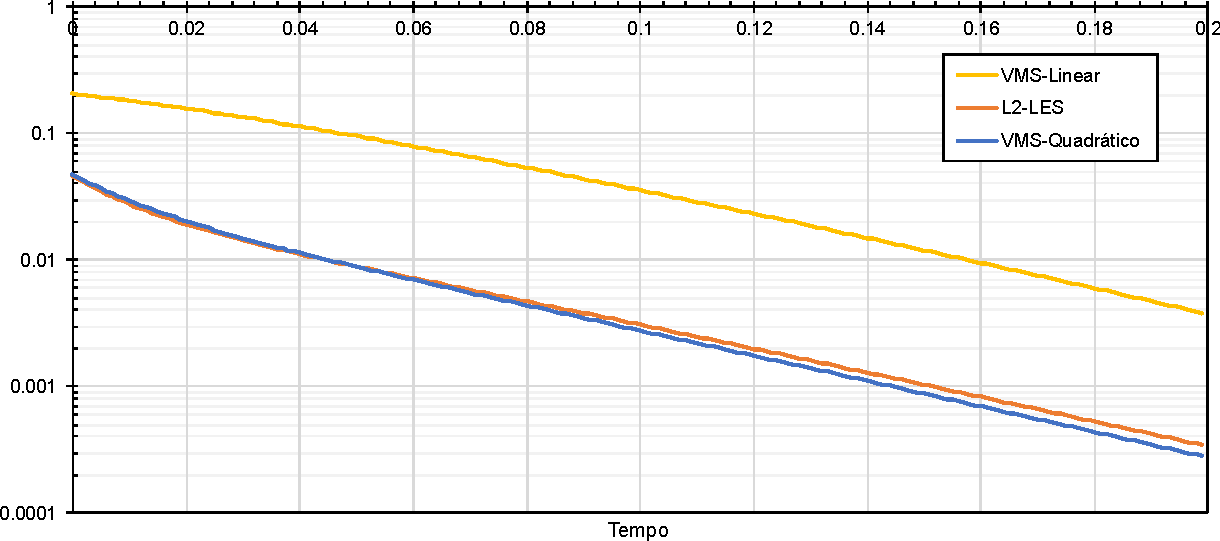
\includegraphics[width=\linewidth]{Figuras/taylor-green/L2.pdf}
    \\Fonte: Autoria Própria (\the\year).
    \label{fig:TGV-L2}
\end{figure}

Assim, observa-se que para o problema estudado, tanto as simulações VMS de aproximação quadrática quanto LES com elemento P2P1 apresentaram boa concordância com o resultado analítico, sendo que ambos apresentaram erros muito próximos entre si, enquanto o VMS de aproximação linear já apresentou um erro maior. Analisando o instante de tempo $t=0.1$ obteve-se um erro $L^2$ de $3,55\times 10^{-2}$, $2,77\times 10^{-3}$ e $3,07\times 10^{-3}$ para as simulações VMS linear, quadrático e LES, respectivamente. Ao verificar a ordem da medida do erro, observa-se que estes valores se encontram próximos ao obtido por \citeonline{zapata2023parallel}. Realizando uma regressão exponencial do tipo \[\norm{\BB{e}}=a\cdot10^{mt}\] para $t\geq 0,1$, encontra-se $m=-9,80$, $m=-10,01$ e $m=-9,60$ para os respectivos modelos.
\end{comment}

\newpage
%==================================================================================================
\subsection{Escoamento em degrau invertido}
%==================================================================================================

O problema de escoamento em degrau invertido é um problema clássico de escoamento em dutos, sendo bastante utilizado como \textit{benchmark} \cite{armaly1983experimental,chiang1999numerical}. O problema consiste em um escoamento advindo de um duto, cuja seção sofre um alargamento abrupto, conforme ilustrado na Figura \ref{fig:step}. Tal problema tem sua origem nos estudos experimentais de \citeonline{armaly1983experimental} e posteriormente estudado numericamente em problemas tridimensionais por \citeonline{chiang1999numerical}.

\begin{figure}[h!]
    \centering
    \caption{Escoamento em degrau invertido - Desenho esquemático.}
    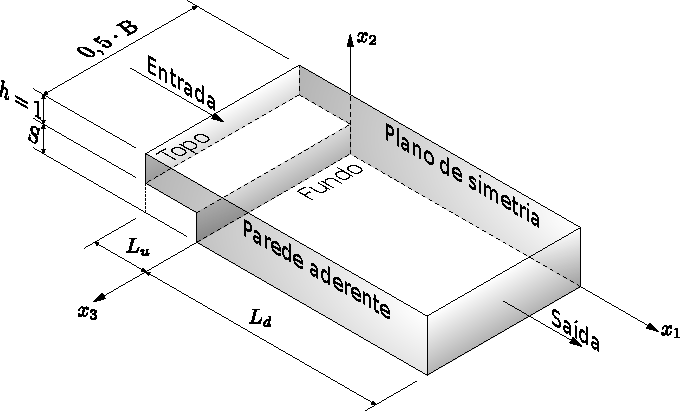
\includegraphics[width=.7\linewidth]{Figuras/backwardFacingStep/backwardFacingStep.pdf}
    \\Fonte: Autoria Própria (\the\year).
    \label{fig:step}
\end{figure}

Em seu estudo numérico, \citeonline{chiang1999numerical} considerou um duto de largura constante $B$, uma altura de seção transversal a montante de $h$ e comprimento $L_u$, e altura a jusante de $H=h+S$ com comprimento $L_d$. Nas laterais do duto considerou-se paredes aderentes, ou seja, $\BB{u}=\BB{0}$, assim como nas faces do fundo e do topo do duto. Na face de entrada do duto considerou-se uma velocidade prescrita $\BB{u}_\infty=(u_1(x_2,x_3),0,0)\trans$, tal que:

\begin{subequations}
    \begin{equation}
        u_1(x_2,x_3)=\frac{48}{\alpha\pi^3}\beta(x_1,x_2)\text{,}
    \end{equation}
    \begin{equation}
        \alpha=1-\frac{192B}{\pi^5}\sum_{i=1,3,5,\hdots}^{\infty}\frac{\tanh{(\xi_i)}}{i^5}\text{,}
    \end{equation}
    \begin{equation}
        \beta(x_1,x_2)=\sum_{i=1,3,5,\hdots}^{\infty}(-1)^{(i-1)/2}\bigpar{1-\frac{\cosh{[(2x_2-1)\xi_i]}}{\cosh{(\xi_i)}}}\frac{\cos{(2x_3\xi_i)}}{i^3}\text{ e}
    \end{equation}
    \begin{equation}
        \xi_i=\frac{\pi i}{2B}\text{.}
    \end{equation}
\end{subequations}

Devido à simetria do problema, considerou-se somente metade da largura do duto, impondo-se uma condição de simetria ($u_3=0$) no plano $x_3=0$, o qual é utilizado para observar os resultados do problema.

Para a simulação numérica, considerou-se um duto com largura $B=35h$, altura $h=1,0$, altura do degrau $S=0,9423$ e comprimento $L_u=0,0$ e $L_d=55,0$. A malha utilizada na discretização do domínio foi construída a partir de elementos tetraédicos de aproximação quadrática e P2P1 de tamanho 0,5 na região de entrada do duto e 0,6 na região de saída. Assim obtém-se uma malha com 57173 elementos finitos, tendo 95334 nós para elementos quadráticos e 95334 nós para o campo de velocidades e 14227 nós para pressões em elementos P2P1, resultando em 381336 e 300229 graus de liberdade, respectivamente (conforme ilustrado na Figura \ref{fig:step-mesh}).

\begin{figure}
    \centering
    \caption{Escoamento em degrau invertido - Malha utilizada.}
    \begin{subfigure}{\textwidth}
        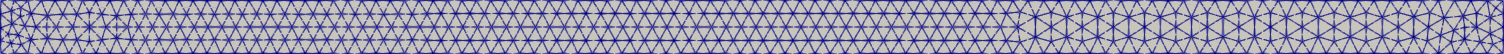
\includegraphics[width=\linewidth]{Figuras/backwardFacingStep/malha1.png}
        \caption{Vista lateral.}
    \end{subfigure}
    \begin{subfigure}{\textwidth}
        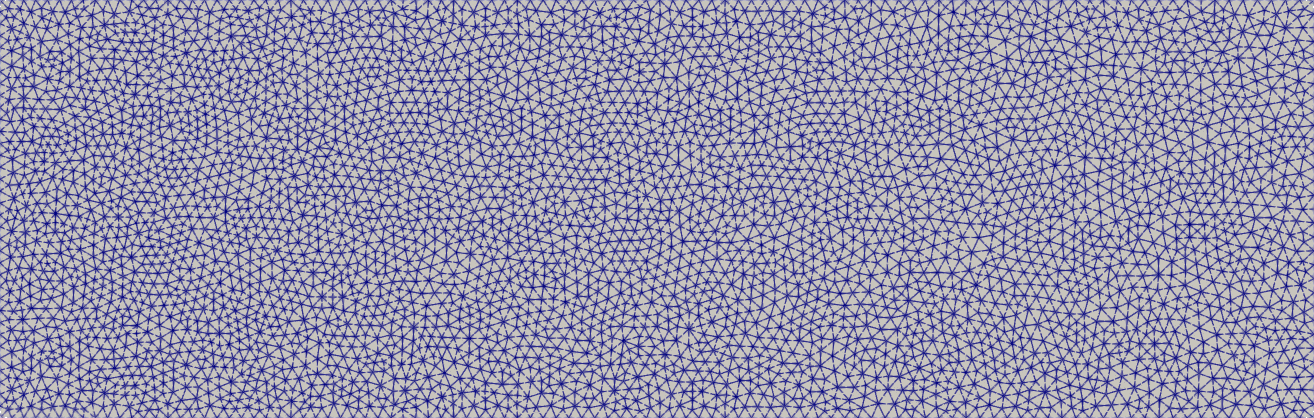
\includegraphics[width=\linewidth]{Figuras/backwardFacingStep/malha2.png}
        \caption{Vista superior.}
    \end{subfigure}
    \\Fonte: Autoria Própria (\the\year).
    \label{fig:step-mesh}
\end{figure}

O número de Reynolds do problema analisado é obtido a partir da equação \eqref{eq:ReyBFS}:

\begin{equation}
    \Rey=\frac{\rho u_\mathrm{médio}(2h)}{\mu}\text{,}
    \label{eq:ReyBFS}
\end{equation}

\noindent sendo $u_\mathrm{médio}=1,0$ a velocidade média na região de entrada do duto. Assim, sendo $\rho=1,0$, considera-se os valores de viscosidade dinâmica $\mu=0,02$, $5,1414\times10^{-3}$ e $2,0\times10^{-3}$, o que resulta em $\Rey=100$, $389$ e $1000$, respectivamente. O passo de tempo foi de $\Delta t=0,1$ e a simulação foi mantida até que a estacionariedade do fluxo fosse alcançada, sendo o esquema de integração temporal obtido a partir de $\rho_\infty=0,0$. A simulação com elementos quadráticos foi estabilizada a partir da formulação SUPG/PSPG, enquanto a simulação P2P1 não foi estabilizada para $\Rey=100$ e $389$, uma vez que a simulação se tornou instável para $\Rey=1000$, sendo, portanto, necessária a aplicação de uma estabilização SUPG nesse caso.

Além disso, uma simulação bidimensional foi conduzida para o $\Rey=1000$, uma vez que \citeonline{chiang1999numerical} observaram uma discrepância entre os valores de simulações bidimensionais e tridimensionais para esse número de Reynolds. Como mencionado pelos autores, essa diferença se dá pela influência da parede aderente nos resultados, o que não é capturada pela simulação bidimensional.

A malha utilizada para a simulação bidimensional foi construída a partir de elementos triangulares de aproximação quadrática de tamanho 0,5 na região de entrada do duto e 0,6 na região de saída. Assim obtém-se uma malha com 836 elementos finitos e 1883 nós, resultando em 5649 graus de liberdade.

A Figura \ref{fig:BFSvel} apresenta os perfis de velocidade para diferentes distâncias ao longo da linha de fluxo para as três simulações conduzidas. Já a Figura \ref{fig:BFSpre} apresenta as distribuições de pressão ao longo do fundo e do topo do duto para as três simulações.

\begin{figure}[h!]
    \centering
    \caption{Escoamento em degrau invertido - Perfis de velocidade.}
    \begin{subfigure}{0.9\textwidth}
        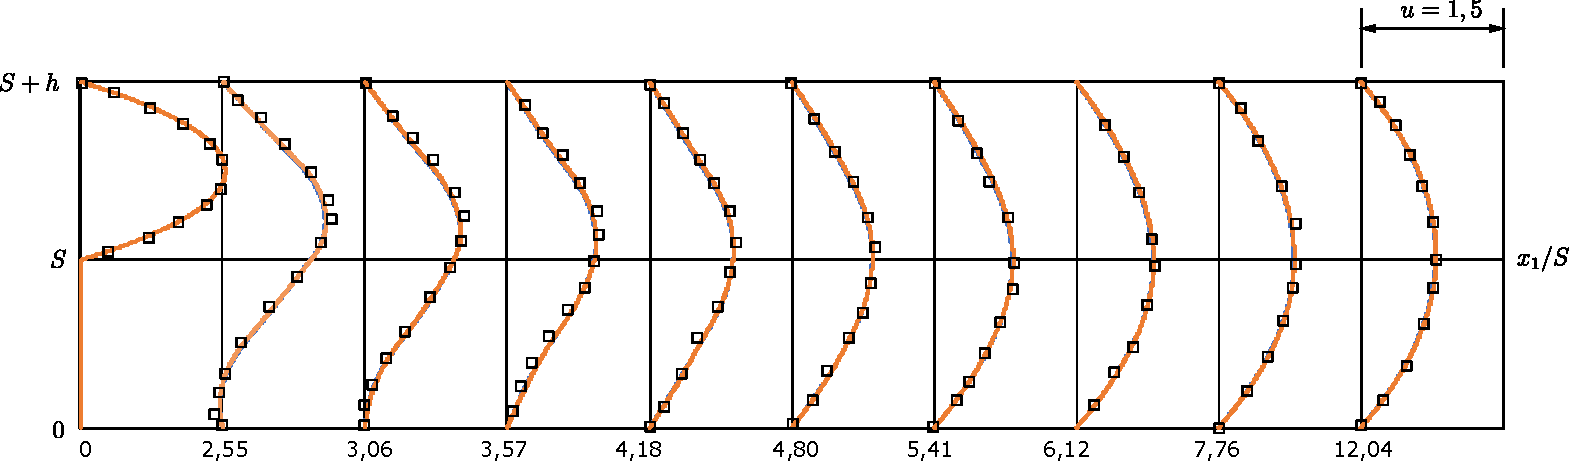
\includegraphics[width=\linewidth]{Figuras/backwardFacingStep/Re100.pdf}
        \caption{$\Rey=100$}
    \end{subfigure}
    \begin{subfigure}{0.9\textwidth}
        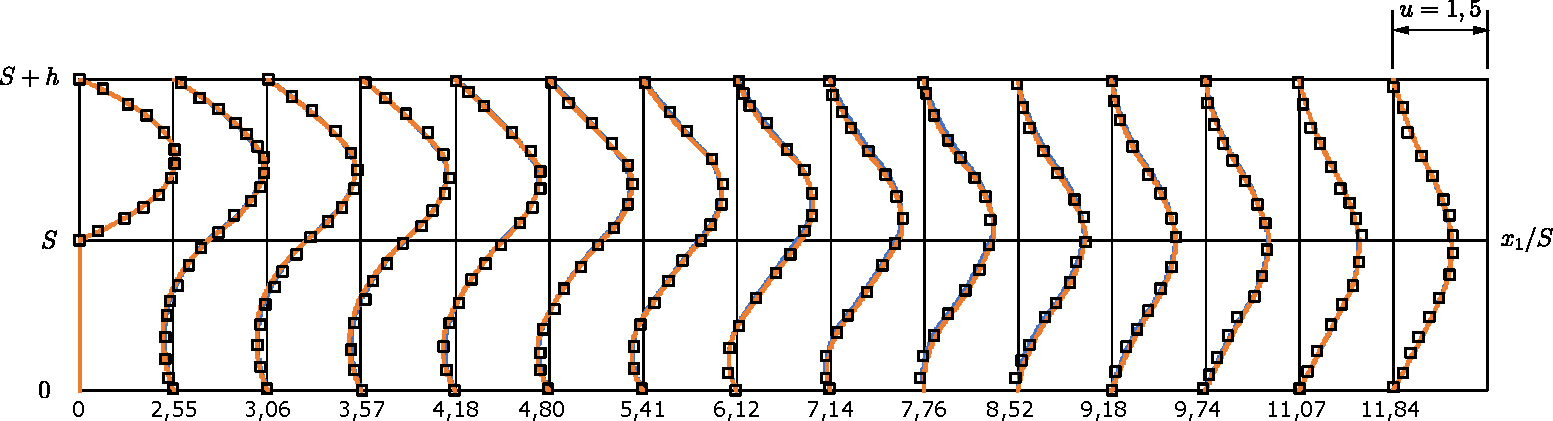
\includegraphics[width=\linewidth]{Figuras/backwardFacingStep/Re389.pdf}
        \caption{$\Rey=389$}
    \end{subfigure}
    \begin{subfigure}{0.9\textwidth}
        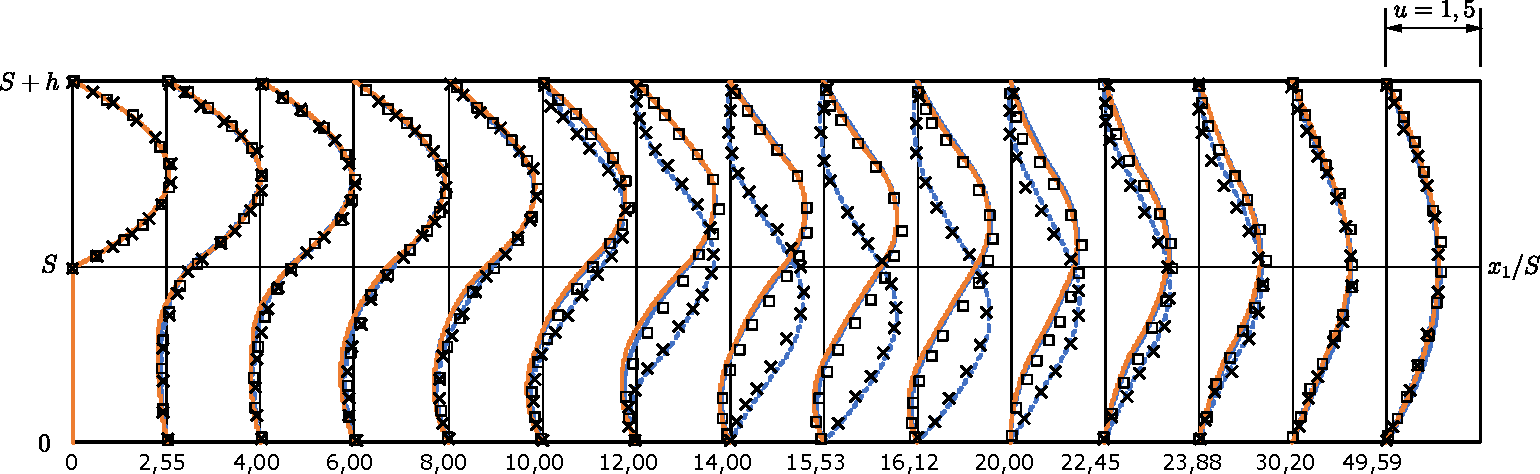
\includegraphics[width=\linewidth]{Figuras/backwardFacingStep/Re1000.pdf}
        \caption{$\Rey=1000$}
    \end{subfigure}
    \begin{subfigure}{0.3\textwidth}
        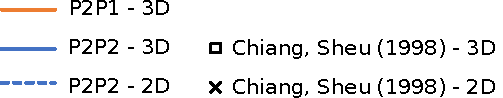
\includegraphics[width=\linewidth]{Figuras/backwardFacingStep/legenda.pdf}
    \end{subfigure}
    \\Fonte: Autoria Própria (\the\year).
    \label{fig:BFSvel}
\end{figure}

\begin{figure}[h!]
    \centering
    \caption{Escoamento em degrau invertido - Distribuição de pressões.}
    \begin{subfigure}{0.65\textwidth}
        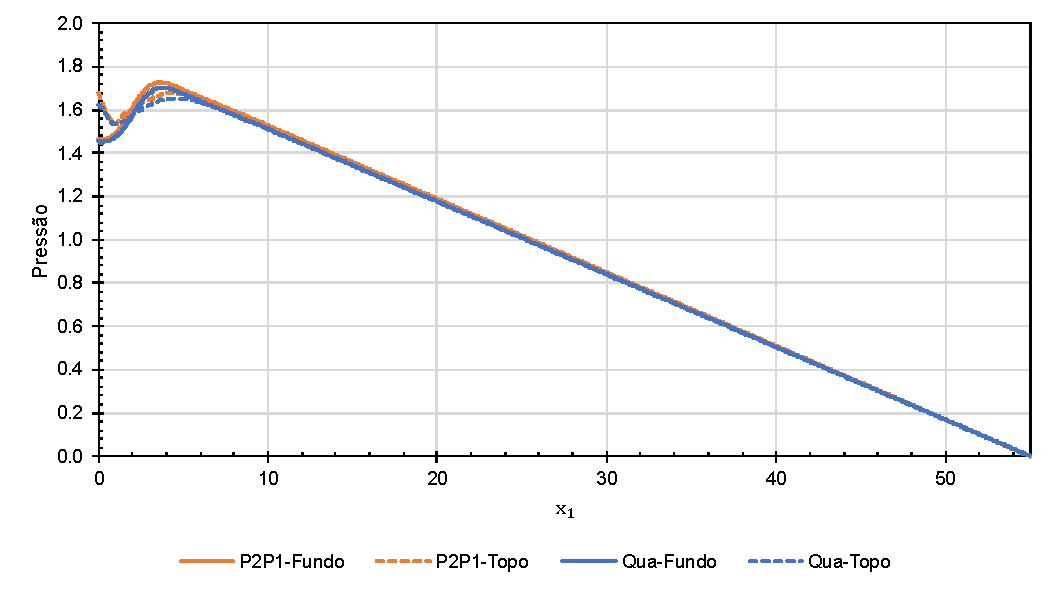
\includegraphics[width=\linewidth]{Figuras/backwardFacingStep/pre100.pdf}
        \caption{$\Rey=100$}
    \end{subfigure}
    \begin{subfigure}{0.65\textwidth}
        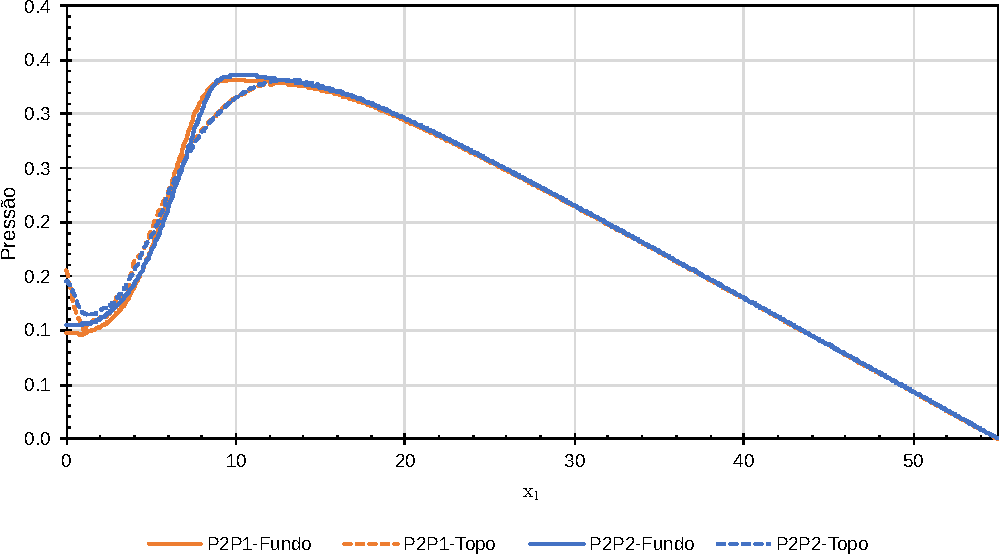
\includegraphics[width=\linewidth]{Figuras/backwardFacingStep/pre389.pdf}
        \caption{$\Rey=389$}
    \end{subfigure}
    \begin{subfigure}{0.65\textwidth}
        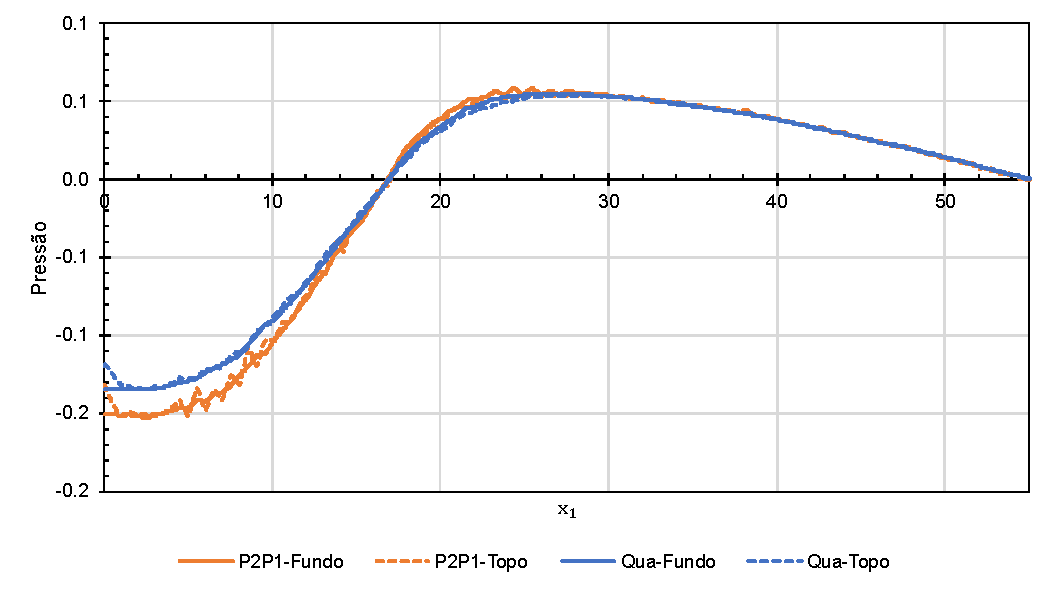
\includegraphics[width=\linewidth]{Figuras/backwardFacingStep/pre1000.pdf}
        \caption{$\Rey=1000$}
    \end{subfigure}
    \\Fonte: Autoria Própria (\the\year).
    \label{fig:BFSpre}
\end{figure}

Outra simulação realizada trata-se do problema bidimensional com $S=1$ e $\Rey=800$, onde os autores observaram os perfis de velocidade para as distâncias $x_1=14$ e $x_1=30$, além da distribuição de pressões ao longo do fundo e do topo do canal. Como a pressão de estagnação do problema simulado é nula na face de saída do duto, foi apenas adicionada uma pressão constante nos resultados de referência para fins de comparação, de forma que as pressões sejam equivalentes nesse ponto especificado. As Figuras \ref{fig:BFS800-vel} e \ref{fig:BFS800-pre} apresentam os resultados obtidos para a simulação bidimensional.

\begin{figure}[h!]
    \centering
    \caption{Escoamento em degrau invertido - Perfis de velocidade para $\Rey=800$.}
    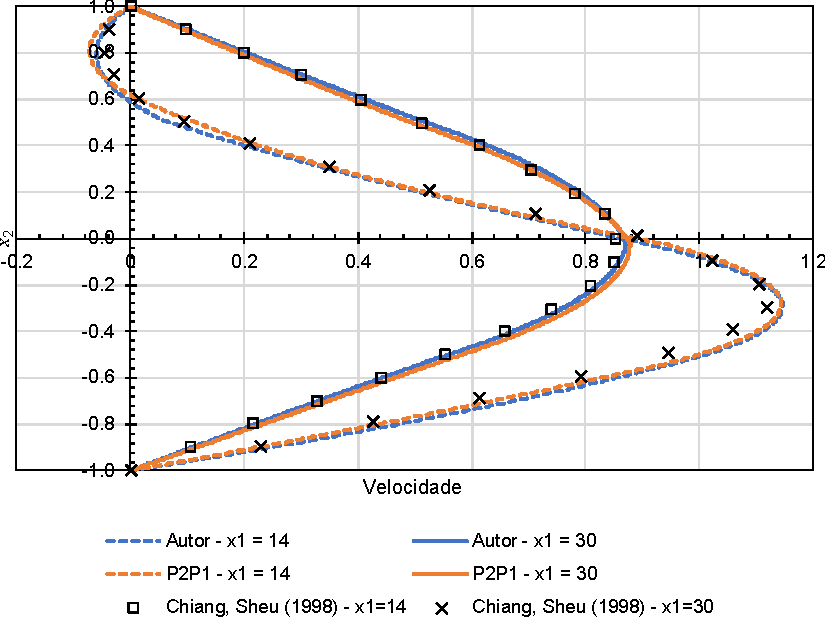
\includegraphics[width=.6\linewidth]{Figuras/backwardFacingStep/resultado2D-2.pdf}
    \\Fonte: Autoria Própria (\the\year).
    \label{fig:BFS800-vel}
\end{figure}

\begin{figure}[h!]
    \centering
    \caption{Escoamento em degrau invertido - Distribuição de pressões para $\Rey=800$.}
    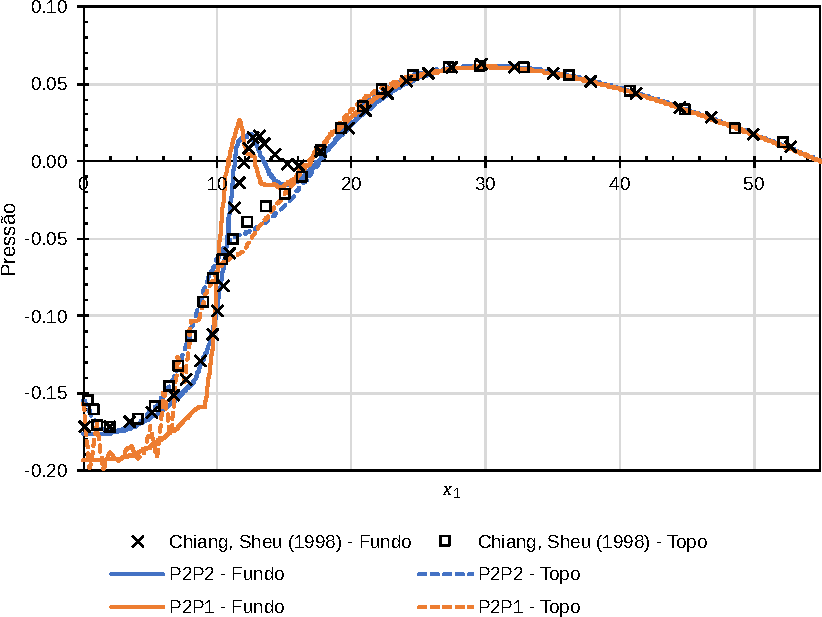
\includegraphics[width=.6\linewidth]{Figuras/backwardFacingStep/resultado2D-1.pdf}
    \\Fonte: Autoria Própria (\the\year).
    \label{fig:BFS800-pre}
\end{figure}

Assim, percebe-se que, em relação ao campo de velocidades, todas as simulações possuíram resultados satisfatórios em todos os números de Reynolds analisados, tanto em simulações bidimensionais quanto tridimensionais. No entanto, para o campo de pressões, observa-se que os elementos P2P1 apresentaram oscilações espúrias, principalmente próximo à face de entrada, o que não é observado na simulação estabilizada por PSPG.

%==================================================================================================
\subsection{Escoamento sobre cilindro}
%==================================================================================================

Para o seguinte problema considerou-se um cilindro circular de raio $R=0,5$ em um domínio retangular $\Omega=[0,112R]\times[0,100R]$, sendo o centro do cilindro posicionado sobre o ponto $(36,50)R$. As condições de contorno consideradas foram de entrada na face esquerda ($x_1=0$) do domínio ($\BB{u}=\{u_\infty,0\}^T$) e condição de velocidade vertical nula nas faces inferior e superior ($u_2=0$ em $x_2=0$ e $x_2=100R$). Como condição inicial aplicou-se uma velocidade $\BB{u}=\{u_\infty,0\}^T$ em todo o domínio. A densidade do fluido foi de $\rho=1,0$ e a velocidade $u_\infty=1,0$. A viscosidade dinâmica do fluido foi de $\nu=0,01$, $\nu=6,6667\times10^{-3}$ e $\nu=5\times10^{-3}$, de forma a se obter $\Rey=100$, $\Rey=150$ e $\Rey=200$, respectivamente.

Para a simulação numérica considerou-se a malha apresentada na Figura \ref{fig:cyl-mesh}, a qual possui 4656 elementos finitos. Assim, estudou-se o escoamento nas simulações apresentadas na Tabela \ref{tab:cyl-sim}. O intervalo de tempo foi de $t\in[0,200]$ com passos de $\Delta t=0,1$.

\begin{figure}[h!]
    \centering
    \caption{Escoamento sobre cilindro - Malha utilizada.}
    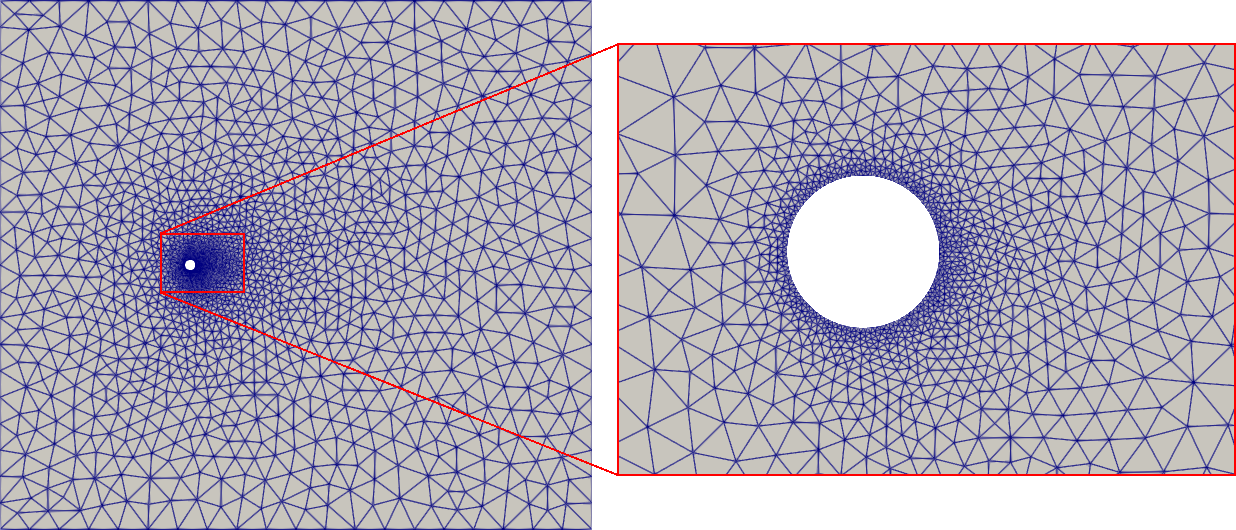
\includegraphics[width=\linewidth]{Figuras/cylinder/analise2/mesh.png}
    \\Fonte: Autoria Própria (\the\year).
    \label{fig:cyl-mesh}
\end{figure}

\begin{table}[h!]
    \centering
    \caption{Simulações conduzidas para o problema de escoamento sobre um cilindro.}
    \begin{tabular}{llllc}
        \hline
        Nome & Modelo & Elemento   & Estabilização & Número de DOF \\\hline
        DNS1 & DNS    & P2P1       & -             & 21417         \\
        DNS2 & DNS    & Quadrático & SUPG/PSPG     & 28494         \\
        DNS3 & DNS    & Quadrático & VMS           & 28494         \\
        LES1 & LES    & P2P1       & -             & 21417         \\
        LES2 & LES    & Quadrático & VMS           & 28494         \\\hline
    \end{tabular}
    \\Fonte: Autoria Própria (\the\year).
    \label{tab:cyl-sim}
\end{table}

Para análise dos resultados determinou-se os coeficientes de arrasto (\textit{Drag} - $C_D$) e de sustentação (\textit{Lift} - $C_L$), dados respectivamente por:

\begin{subequations}
    \begin{equation}
        C_D=\frac{2F_D}{\rho\norm{\BB{u}_\infty}^2L}\text{ e}
    \end{equation}
    \begin{equation}
        C_L=\frac{2F_L}{\rho\norm{\BB{u}_\infty}^2L}\text{,}
    \end{equation}
\end{subequations}

\noindent em que $F_D$ e $F_L$ são as forças de arrasto e de sustentação, calculados como:

\begin{subequations}
    \begin{equation}
        F_D=\int_{\Gamma_S}{\sigma_{1j}n_jd\Gamma_S}\text{ e}
    \end{equation}
    \begin{equation}
        F_L=\int_{\Gamma_S}{\sigma_{2j}n_jd\Gamma_S}\text{,}
    \end{equation}
\end{subequations}

\noindent sendo $\Gamma_S$ a fronteira do cilindro e $\BB{n}$ o vetor normal à $\Gamma_S$.

Outro parâmetro possível de se verificar é o número de Strouhal ($\Str$), que se trata de um número adimensional que busca relacionar a frequência de oscilação devido à formação de vórtices e a velocidade do fluido. Esse parâmetro pode ser determinado por:

\begin{equation}
    \Str=\frac{f_vL}{\norm{\BB{u}_\infty}}\text{,}
\end{equation}

\noindent sendo $f_v$ a frequência de desprendimento de vórtices.

As Figuras \ref{fig:cyl-Cd} e \ref{fig:cyl-Cl} apresentam os coeficientes de arrasto e de sustentação obtidos em todas as simulações, respectivamente.

\begin{figure}[h!]
    \centering
    \caption{Escoamento sobre cilindro - Coeficiente de arrasto ao longo do tempo.}
    \begin{subfigure}{\textwidth}
        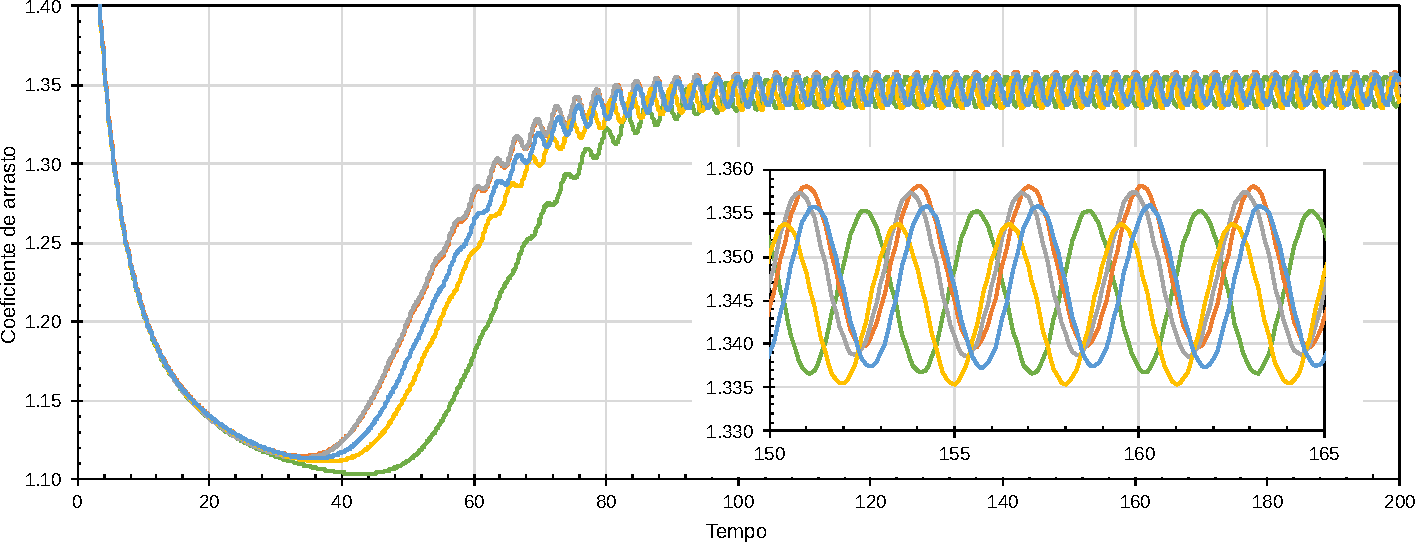
\includegraphics[width=\linewidth]{Figuras/cylinder/analise3/Cd-100.pdf}
        \caption{$\Rey=100$}
    \end{subfigure}
    \begin{subfigure}{\textwidth}
        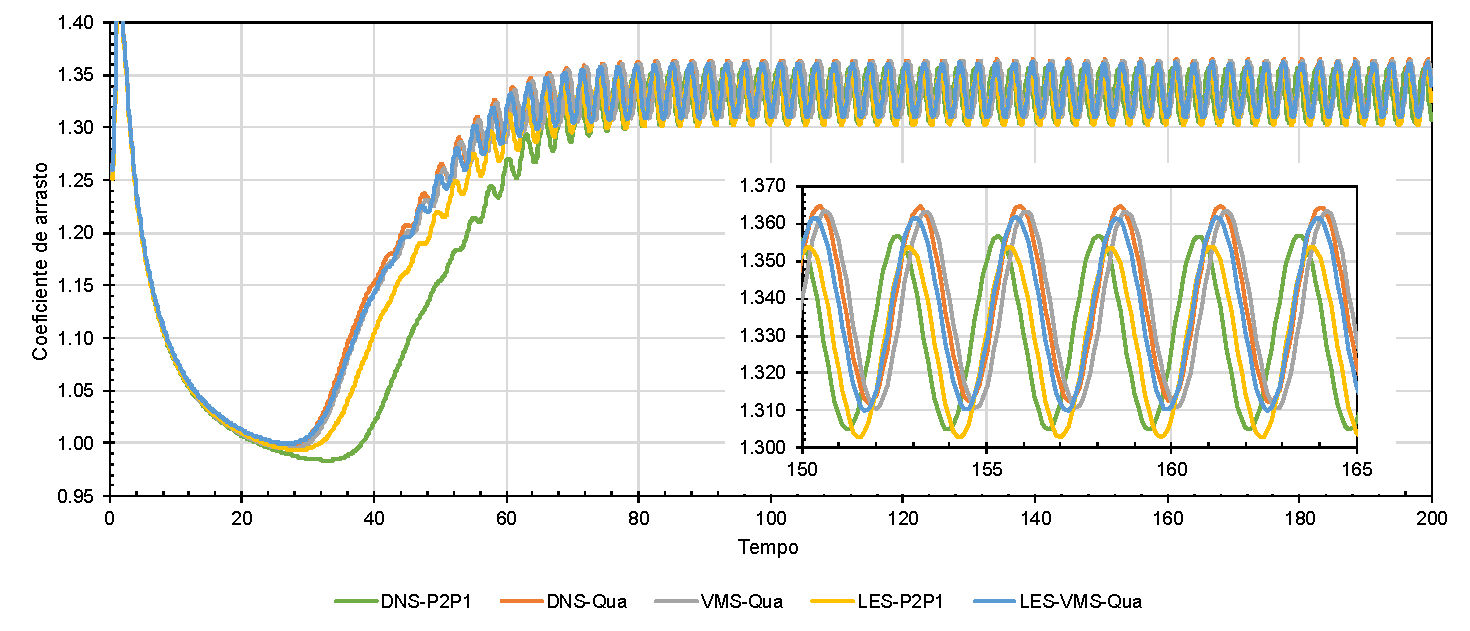
\includegraphics[width=\linewidth]{Figuras/cylinder/analise3/Cd-150.pdf}
        \caption{$\Rey=150$}
    \end{subfigure}
    \begin{subfigure}{\textwidth}
        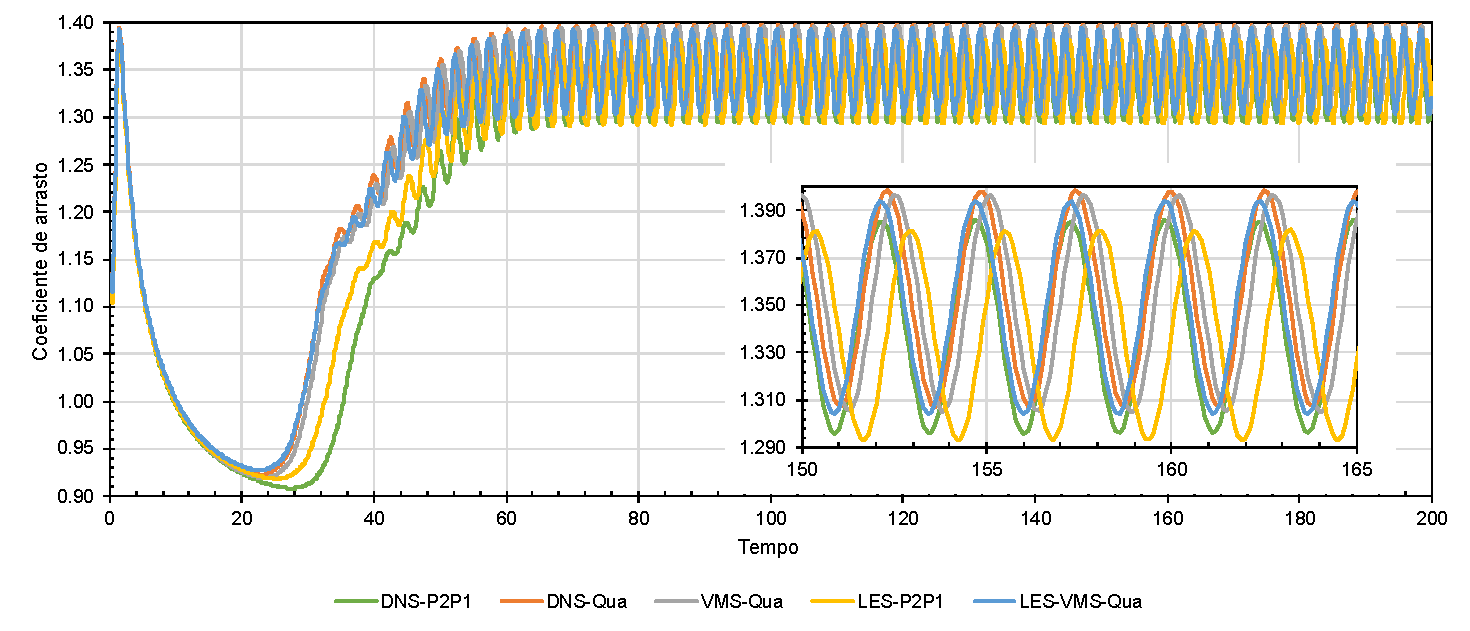
\includegraphics[width=\linewidth]{Figuras/cylinder/analise3/Cd-200.pdf}
        \caption{$\Rey=200$}
    \end{subfigure}
    \\Fonte: Autoria Própria (\the\year).
    \label{fig:cyl-Cd}
\end{figure}
\newpage

\begin{figure}[h!]
    \centering
    \caption{Escoamento sobre cilindro - Coeficiente de sustentação ao longo do tempo.}
    \begin{subfigure}{\textwidth}
        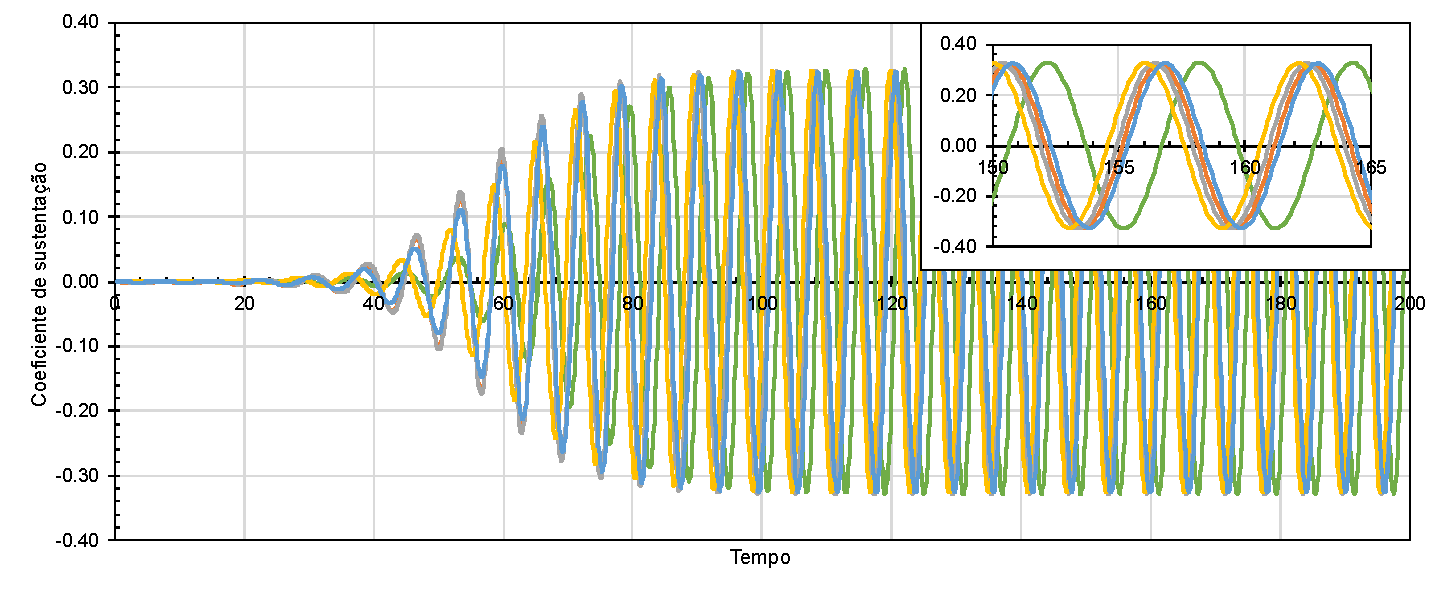
\includegraphics[width=\linewidth]{Figuras/cylinder/analise3/Cl-100.pdf}
        \caption{$\Rey=100$}
    \end{subfigure}
    \begin{subfigure}{\textwidth}
        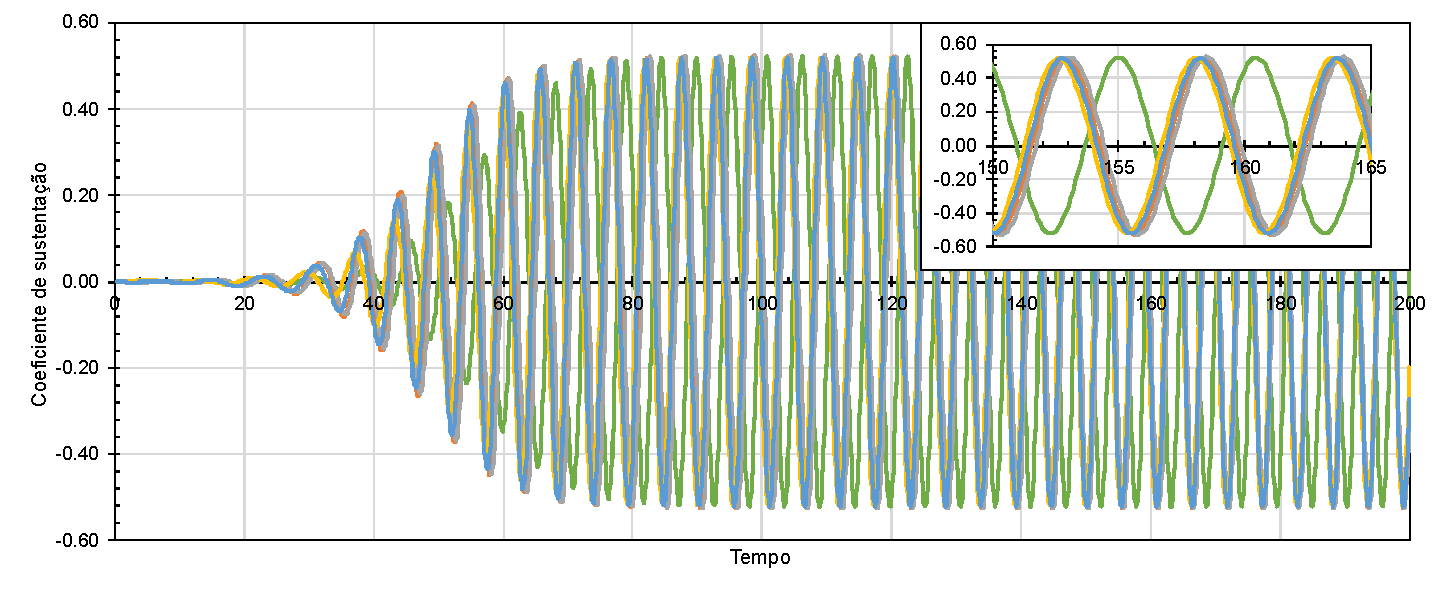
\includegraphics[width=\linewidth]{Figuras/cylinder/analise3/Cl-150.pdf}
        \caption{$\Rey=150$}
    \end{subfigure}
    \begin{subfigure}{\textwidth}
        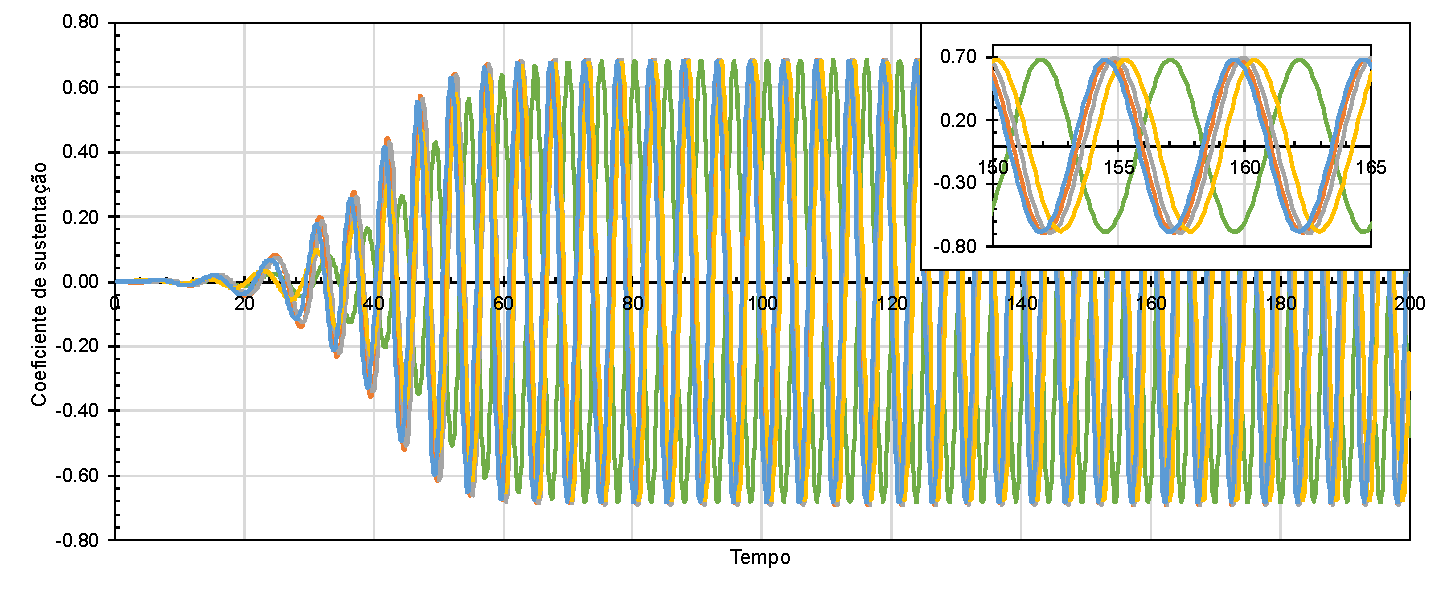
\includegraphics[width=\linewidth]{Figuras/cylinder/analise3/Cl-200.pdf}
        \caption{$\Rey=200$}
    \end{subfigure}
    \\Fonte: Autoria Própria (\the\year).
    \label{fig:cyl-Cl}
\end{figure}
\newpage

Os valores dos coeficientes de arrasto e de sustentação após o escoamento atingir o equilíbrio dinâmico, assim como o número de Strouhal e valores de referência, são apresentados nas Tabelas \ref{tab:cyl-res100} a \ref{tab:cyl-res200}.

\begin{table}[h!]
    \centering
    \caption{Escoamento sobre cilindro - Valores dos coeficientes e número de Strouhal para $\Rey=100$.}
    \begin{tabular}{lcccc}
        \hline
        Simulação                          & $C_D$             & $C_L$       & $\Str$   \\\hline
        DNS1                               & $1,3458\pm0,0095$ & $\pm0,3283$ & $0,1642$ \\
        DNS2                               & $1,3488\pm0,0094$ & $\pm0,3255$ & $0,1647$ \\
        DNS3                               & $1,3480\pm0,0095$ & $\pm0,3279$ & $0,1650$ \\
        LES1                               & $1,3445\pm0,0093$ & $\pm0,3264$ & $0,1639$ \\
        LES2                               & $1,3466\pm0,0094$ & $\pm0,3259$ & $0,1646$ \\\hline
        \citeonline{fernandes2020tecnica}  & $1,3700\pm0,0098$ & $\pm0,3422$ & $0,165$  \\
        \citeonline{najafi2012meshless}    & $1,47$            & $\pm0,38$   &          \\
        \citeonline{ji2012novel}           & $1,4643\pm0,0107$ & $\pm0,3351$ & $0,1675$ \\
        \citeonline{liu1998preconditioned} & $1,350\pm0,012$   & $\pm0,339$  & $0,165$  \\\hline
    \end{tabular}
    \\Fonte: Autoria Própria (\the\year).
    \label{tab:cyl-res100}
\end{table}

\begin{table}[h!]
    \centering
    \caption{Escoamento sobre cilindro - Valores dos coeficientes e número de Strouhal para $\Rey=150$.}
    \begin{tabular}{lcccc}
        \hline
        Simulação                          & $C_D$             & $C_D$       & $\Str$   \\\hline
        DNS1                               & $1,3309\pm0,0262$ & $\pm0,5218$ & $0,1848$ \\
        DNS2                               & $1,3384\pm0,0263$ & $\pm0,5231$ & $0,1852$ \\
        DNS3                               & $1,3369\pm0,0265$ & $\pm0,5253$ & $0,1855$ \\
        LES1                               & $1,3283\pm0,0257$ & $\pm0,5184$ & $0,1843$ \\
        LES2                               & $1,3358\pm0,0259$ & $\pm0,5196$ & $0,1847$ \\\hline
        \citeonline{najafi2012meshless}    & $1,45$            & $\pm0,56$   &          \\
        \citeonline{ji2012novel}           & $1,4463\pm0,0261$ & $\pm0,5043$ & $0,1837$ \\
        \citeonline{liu1998preconditioned} & $1,334\pm0,030$   & $\pm0,530$  & $0,182$  \\\hline
    \end{tabular}
    \\Fonte: Autoria Própria (\the\year).
    \label{tab:cyl-res150}
\end{table}

\begin{table}[h!]
    \centering
    \caption{Escoamento sobre cilindro - Valores dos coeficientes e número de Strouhal para $\Rey=200$.}
    \begin{tabular}{lcccc}
        \hline
        Simulação                          & $C_D$             & $C_L$       & $\Str$   \\\hline
        DNS1                               & $1,3409\pm0,0450$ & $\pm0,6833$ & $0,1987$ \\
        DNS2                               & $1,3527\pm0,0456$ & $\pm0,6874$ & $0,1998$ \\
        DNS3                               & $1,3506\pm0,0457$ & $\pm0,6892$ & $0,2001$ \\
        LES1                               & $1,3374\pm0,0442$ & $\pm0,6784$ & $0,1980$ \\
        LES2                               & $1,3490\pm0,0449$ & $\pm0,6825$ & $0,1990$ \\\hline
        \citeonline{fernandes2020tecnica}  & $1,3787\pm0,0476$ & $\pm0,7134$ & $0,195$  \\
        \citeonline{najafi2012meshless}    & $1,46$            & $\pm0,72$   &          \\
        \citeonline{ji2012novel}           & $1,4372\pm0,0417$ & $\pm0,6272$ & $0,1963$ \\
        \citeonline{liu1998preconditioned} & $1,31\pm0,049$    & $\pm0,69$   & $0,192$  \\\hline
    \end{tabular}
    \\Fonte: Autoria Própria (\the\year).
    \label{tab:cyl-res200}
\end{table}

Assim, observa-se que todos os valores estão próximos aos valores de referência, sendo que as simulações baseadas em elementos P2P1 apresentaram valores ligeiramente inferiores aos demais conforme o número de Reynolds aumenta. A mínima diferença observada entre os valores calculados em uma simulação DNS e aquela que em simulação LES deve-se ao fato do número de Reynolds ser muito baixo, pois, como apontado por \citeonline{fernandes2020tecnica}, esse tipo de escoamento (com $\Rey$ entre 50 e 200) apresenta a formação de vórtices laminares, denominada de esteira de Von Kárman.

Em seguida partiu-se para uma análise com a consideração de uma malha mais grosseira, a qual é apresentada na Figura \ref{fig:cyl-mesh2}. A malha utilizada para a simulação foi construída a partir de elementos triangulares, possuindo 5004 graus de liberdade para a simulação de elementos quadráticos e 3771 para a simulação de elementos P2P1. Os valores dos coeificentes de arrasto e de sustentação são apresentados nas Figuras \ref{fig:cyl-Cd2} e \ref{fig:cyl-Cl2}, respectivamente. A linha de referência é considerada como a obtida pela simulação LES-VMS da malha fina.

\begin{figure}[h!]
    \centering
    \caption{Escoamento sobre cilindro - Malha utilizada para simulação com malha mais grosseira.}
    \includegraphics[width=.75\linewidth]{Figuras/cylinder/coarse/mesh.png}
    \\Fonte: Autoria Própria (\the\year).
    \label{fig:cyl-mesh2}
\end{figure}

\begin{figure}[h!]
    \centering
    \caption{Escoamento sobre cilindro - Coeficiente de arrasto ao longo do tempo para malha mais grosseira.}
    \begin{subfigure}{\textwidth}
        \centering
        \includegraphics[width=.85\linewidth]{Figuras/cylinder/coarse/Cd100.pdf}
        \caption{$\Rey=100$}
    \end{subfigure}
    \begin{subfigure}{\textwidth}
        \centering
        \includegraphics[width=.85\linewidth]{Figuras/cylinder/coarse/Cd150.pdf}
        \caption{$\Rey=150$}
    \end{subfigure}
    \begin{subfigure}{\textwidth}
        \centering
        \includegraphics[width=.85\linewidth]{Figuras/cylinder/coarse/Cd200.pdf}
        \caption{$\Rey=200$}
    \end{subfigure}
    \\Fonte: Autoria Própria (\the\year).
    \label{fig:cyl-Cd2}
\end{figure}

\begin{figure}[h!]
    \centering
    \caption{Escoamento sobre cilindro - Coeficiente de sustentação ao longo do tempo para malha mais grosseira.}
    \begin{subfigure}{\textwidth}
        \includegraphics[width=\linewidth]{Figuras/cylinder/coarse/Cl100.pdf}
        \caption{$\Rey=100$}
    \end{subfigure}
    \begin{subfigure}{\textwidth}
        \includegraphics[width=\linewidth]{Figuras/cylinder/coarse/Cl150.pdf}
        \caption{$\Rey=150$}
    \end{subfigure}
    \begin{subfigure}{\textwidth}
        \includegraphics[width=\linewidth]{Figuras/cylinder/coarse/Cl200.pdf}
        \caption{$\Rey=200$}
    \end{subfigure}
    \\Fonte: Autoria Própria (\the\year).
    \label{fig:cyl-Cl2}
\end{figure}

Os valores dos coeficientes de arrasto e de sustentação após o escoamento atingir o equilíbrio dinâmico, assim como o número de Strouhal e valores obtidos na simulação com malha fina, são apresentados na Tabela \ref{tab:cyl-comp100} a \ref{tab:cyl-comp200}.

\begin{table}[h!]
    \centering
    \caption{Escoamento sobre cilindro - Comparação de $C_D$, $C_L$ e $\Str$ para $\Rey=100$.}
    \begin{tabular}{lcccccc}
        \hline
        \multirow{2}{*}{Simulação} & \multicolumn{3}{c}{Malha 1} & \multicolumn{3}{c}{Malha 2}                                                         \\\cline{2-7}
                                   & $C_D$                       & $C_L$                       & $\Str$   & $C_D$             & $C_L$       & $\Str$   \\\hline
        DNS1                       & $1,3458\pm0,0095$           & $\pm0,3283$                 & $0,1642$ & $1,1913\pm0,0120$ & $\pm0,2966$ & $0,1464$ \\
        DNS2                       & $1,3488\pm0,0094$           & $\pm0,3255$                 & $0,1647$ & $1,3502\pm0,0128$ & $\pm0,3637$ & $0,1614$ \\
        DNS3                       & $1,3480\pm0,0095$           & $\pm0,3279$                 & $0,1650$ & $1,3320\pm0,0136$ & $\pm0,3759$ & $0,1621$ \\
        LES1                       & $1,3445\pm0,0093$           & $\pm0,3264$                 & $0,1639$ & $1,1832\pm0,0103$ & $\pm0,2683$ & $0,1442$ \\
        LES2                       & $1,3466\pm0,0094$           & $\pm0,3259$                 & $0,1646$ & $1,3210\pm0,0121$ & $\pm0,3527$ & $0,1589$ \\\hline
    \end{tabular}
    \\Fonte: Autoria Própria (\the\year).
    \label{tab:cyl-comp100}
\end{table}

\begin{table}[h!]
    \centering
    \caption{Escoamento sobre cilindro - Comparação de $C_D$, $C_L$ e $\Str$ para $\Rey=150$.}
    \begin{tabular}{lcccccc}
        \hline
        \multirow{2}{*}{Simulação} & \multicolumn{3}{c}{Malha 1} & \multicolumn{3}{c}{Malha 2}                                                         \\\cline{2-7}
                                   & $C_D$                       & $C_L$                       & $\Str$   & $C_D$             & $C_L$       & $\Str$   \\\hline
        DNS1                       & $1,3309\pm0,0262$           & $\pm0,5218$                 & $0,1848$ & $1,2101\pm0,0416$ & $\pm0,5879$ & $0,1661$ \\
        DNS2                       & $1,3384\pm0,0263$           & $\pm0,5231$                 & $0,1852$ & $1,3822\pm0,0364$ & $\pm0,5915$ & $0,1821$ \\
        DNS3                       & $1,3369\pm0,0265$           & $\pm0,5253$                 & $0,1855$ & $1,3660\pm0,0378$ & $\pm0,6059$ & $0,1822$ \\
        LES1                       & $1,3283\pm0,0257$           & $\pm0,5184$                 & $0,1843$ & $1,1952\pm0,0337$ & $\pm0,5433$ & $0,1626$ \\
        LES2                       & $1,3358\pm0,0259$           & $\pm0,5196$                 & $0,1847$ & $1,3491\pm0,0346$ & $\pm0,5768$ & $0,1779$ \\\hline
    \end{tabular}
    \\Fonte: Autoria Própria (\the\year).
    \label{tab:cyl-comp150}
\end{table}

\begin{table}[h!]
    \centering
    \caption{Escoamento sobre cilindro - Comparação de $C_D$, $C_L$ e $\Str$ para $\Rey=200$.}
    \begin{tabular}{lcccccc}
        \hline
        \multirow{2}{*}{Simulação} & \multicolumn{3}{c}{Malha 1} & \multicolumn{3}{c}{Malha 2}                                                         \\\cline{2-7}
                                   & $C_D$                       & $C_L$                       & $\Str$   & $C_D$             & $C_L$       & $\Str$   \\\hline
        DNS1                       & $1,3409\pm0,0450$           & $\pm0,6833$                 & $0,1987$ & $1,2118\pm0,0672$ & $\pm0,7190$ & $0,1776$ \\
        DNS2                       & $1,3527\pm0,0456$           & $\pm0,6874$                 & $0,1998$ & $1,4232\pm0,7477$ & $\pm0,7477$ & $0,1947$ \\
        DNS3                       & $1,3506\pm0,0457$           & $\pm0,6892$                 & $0,2001$ & $1,4108\pm0,7646$ & $\pm0,7646$ & $0,1943$ \\
        LES1                       & $1,3374\pm0,0442$           & $\pm0,6784$                 & $0,1980$ & $1,1997\pm0,6768$ & $\pm0,6768$ & $0,1735$ \\
        LES2                       & $1,3490\pm0,0449$           & $\pm0,6825$                 & $0,1990$ & $1,3887\pm0,7283$ & $\pm0,7283$ & $0,1894$ \\\hline
    \end{tabular}
    \\Fonte: Autoria Própria (\the\year).
    \label{tab:cyl-comp200}
\end{table}

Como pode se observar, os valores obtidos a partir de elementos P2P1 tiveram valores muito abaixo do esperado, principalmente para o coeficiente de arrasto, independentemente da aplicação do LES. Já os valores obtidos a partir de elementos quadráticos apresentaram valores mais próximos aos obtidos na simulação com malha mais fina, em que a aplicação do LES se mostrou eficiente para descrever os coeficientes de arrasto e sustentação a partir de $\Rey=150$. Já o número de Strouhal foi levemente amortecido devido à aplicação do modelo.

%Comparando-se os números de Strouhal calculados com aqueles obtidos por \citeonline{fernandes2020tecnica}, que obteve, para a mesma geometria de domínio e mesmas condições de contorno, um $\Str=0,165$ e amplitude do coeficiente de sustentação de 0,3422, \citeonline{tezduyar1992incompressible}, os quais verificaram $\Str$ entre 0,166 e 0,170, \citeonline{najafi2012meshless}, com valor de 0,182, e \citeonline{codina2006numerical}, com valores entre 0,177 e 0,184. As variações observadas entre os números de Strouhal dos diferentes autores podem ser devidas às diferenças nas dimensões dos domínios utilizados, assim como as diferentes condições de contorno aplicadas por cada um. No entanto ainda observa-se que em todos os casos os valores calculados nas simulações ainda são bem próximos. A mínima diferença observada entre os valores calculados em uma simulação DNS e aquela que em simulação LES deve-se ao fato do número de Reynolds ser muito baixo, pois, como apontado por \citeonline{fernandes2020tecnica}, esse tipo de escoamento (com $\Rey$ entre 50 e 200) apresenta a formação de vórtices laminares, denominada de esteira de Von Kárman. Para uma verificação mais precisa dessa influência, deve-se partir para uma análise tridimensional com número de Reynolds superiores à 200.

%Vale observar ainda que a simulação VMS linear apresentou um amortecimento menor em relação ao início das oscilações, porém converge para valores muito próximos ao quadrático ao longo do tempo. Já a simulação LES inicia sua oscilação próxima ao VMS quadrático, entretanto com uma média de oscilação menor que a do VMS, em especial ao se observar o coeficiente de arrasto. Tal efeito pode ser devido ao relatado por \citeonline{germano1991dynamic,hughes2000large}, que apontam a ocorrência de um amortecimento excessivo provocado pelo tensor SGS de Smagorinsky.
\begin{comment}
\begin{figure}[h!]
    \centering
    \caption{Campos de velocidades e de pressões no instante $t=120$ para elemento de aproximação linear.}
    \begin{subfigure}{\textwidth}
        \begin{subfigure}{\textwidth}\centering
            \begin{subfigure}{.42\textwidth}
                \caption*{Campo de velocidades.}
                \includegraphics[width=\linewidth]{Figuras/cylinder/analise2/lu.png}
            \end{subfigure}
            \begin{subfigure}{.42\textwidth}
                \caption*{Campo de pressões.}
                \includegraphics[width=\linewidth]{Figuras/cylinder/analise2/lp.png}
            \end{subfigure}
        \end{subfigure}
    \end{subfigure}
    \begin{subfigure}{\textwidth}\centering
        \begin{subfigure}{.49\textwidth}
            \includegraphics[width=\linewidth]{Figuras/cylinder/analise2/none-Lin-u.png}
        \end{subfigure}
        \begin{subfigure}{.49\textwidth}
            \includegraphics[width=\linewidth]{Figuras/cylinder/analise2/none-Lin-p.png}
        \end{subfigure}
        \caption{Sem modelo}
    \end{subfigure}
    \begin{subfigure}{\textwidth}\centering
        \begin{subfigure}{.49\textwidth}
            \includegraphics[width=\linewidth]{Figuras/cylinder/analise2/LES-Lin-u.png}
        \end{subfigure}
        \begin{subfigure}{.49\textwidth}
            \includegraphics[width=\linewidth]{Figuras/cylinder/analise2/LES-Lin-p.png}
        \end{subfigure}
        \caption{LES}
    \end{subfigure}
    \begin{subfigure}{\textwidth}\centering
        \begin{subfigure}{.49\textwidth}
            \includegraphics[width=\linewidth]{Figuras/cylinder/analise2/VMS-Lin-u.png}
        \end{subfigure}
        \begin{subfigure}{.49\textwidth}
            \includegraphics[width=\linewidth]{Figuras/cylinder/analise2/VMS-Lin-p.png}
        \end{subfigure}
        \caption{VMS}
    \end{subfigure}
    \\Fonte: Autoria Própria (\the\year).
    \label{fig:vel-pre-Lin}
\end{figure}
\newpage

\begin{figure}[h!]
    \centering
    \caption{Campos de velocidades e de pressões no instante $t=120$ para elemento de aproximação quadrática.}
    \begin{subfigure}{\textwidth}
        \begin{subfigure}{\textwidth}\centering
            \begin{subfigure}{.42\textwidth}
                \caption*{Campo de velocidades.}
                \includegraphics[width=\linewidth]{Figuras/cylinder/analise2/lu.png}
            \end{subfigure}
            \begin{subfigure}{.42\textwidth}
                \caption*{Campo de pressões.}
                \includegraphics[width=\linewidth]{Figuras/cylinder/analise2/lp.png}
            \end{subfigure}
        \end{subfigure}
    \end{subfigure}
    \begin{subfigure}{\textwidth}\centering
        \begin{subfigure}{.49\textwidth}
            \includegraphics[width=\linewidth]{Figuras/cylinder/analise2/none-Qua-u.png}
        \end{subfigure}
        \begin{subfigure}{.49\textwidth}
            \includegraphics[width=\linewidth]{Figuras/cylinder/analise2/none-Qua-p.png}
        \end{subfigure}
        \caption{Sem modelo}
    \end{subfigure}
    \begin{subfigure}{\textwidth}\centering
        \begin{subfigure}{.49\textwidth}
            \includegraphics[width=\linewidth]{Figuras/cylinder/analise2/LES-Qua-u.png}
        \end{subfigure}
        \begin{subfigure}{.49\textwidth}
            \includegraphics[width=\linewidth]{Figuras/cylinder/analise2/LES-Qua-p.png}
        \end{subfigure}
        \caption{LES}
    \end{subfigure}
    \begin{subfigure}{\textwidth}\centering
        \begin{subfigure}{.49\textwidth}
            \includegraphics[width=\linewidth]{Figuras/cylinder/analise2/VMS-Qua-u.png}
        \end{subfigure}
        \begin{subfigure}{.49\textwidth}
            \includegraphics[width=\linewidth]{Figuras/cylinder/analise2/VMS-Qua-p.png}
        \end{subfigure}
        \caption{VMS}
    \end{subfigure}
    \\Fonte: Autoria Própria (\the\year).
    \label{fig:vel-pre-Qua}
\end{figure}
\newpage

\begin{figure}[h!]
    \centering
    \caption{Campos de velocidades e de pressões no instante $t=120$ para elemento Taylor-Hood P2P1.}
    \begin{subfigure}{\textwidth}
        \begin{subfigure}{\textwidth}\centering
            \begin{subfigure}{.42\textwidth}
                \caption*{Campo de velocidades.}
                \includegraphics[width=\linewidth]{Figuras/cylinder/analise2/lu.png}
            \end{subfigure}
            \begin{subfigure}{.42\textwidth}
                \caption*{Campo de pressões.}
                \includegraphics[width=\linewidth]{Figuras/cylinder/analise2/lp.png}
            \end{subfigure}
        \end{subfigure}
    \end{subfigure}
    \begin{subfigure}{\textwidth}\centering
        \begin{subfigure}{.49\textwidth}
            \includegraphics[width=\linewidth]{Figuras/cylinder/analise2/none-TH-u.png}
        \end{subfigure}
        \begin{subfigure}{.49\textwidth}
            \includegraphics[width=\linewidth]{Figuras/cylinder/analise2/none-TH-p.png}
        \end{subfigure}
        \caption{Sem modelo}
    \end{subfigure}
    \begin{subfigure}{\textwidth}\centering
        \begin{subfigure}{.49\textwidth}
            \includegraphics[width=\linewidth]{Figuras/cylinder/analise2/LES-TH-u.png}
        \end{subfigure}
        \begin{subfigure}{.49\textwidth}
            \includegraphics[width=\linewidth]{Figuras/cylinder/analise2/LES-TH-p.png}
        \end{subfigure}
        \caption{LES}
    \end{subfigure}
    \begin{subfigure}{\textwidth}\centering
        \begin{subfigure}{.49\textwidth}
            \includegraphics[width=\linewidth]{Figuras/cylinder/analise2/VMS-TH-u.png}
        \end{subfigure}
        \begin{subfigure}{.49\textwidth}
            \includegraphics[width=\linewidth]{Figuras/cylinder/analise2/VMS-TH-p.png}
        \end{subfigure}
        \caption{VMS}
    \end{subfigure}
    \\Fonte: Autoria Própria (\the\year).
    \label{fig:vel-pre-TH}
\end{figure}
\newpage
\end{comment}

\newpage
%==================================================================================================
\subsection{Escoamento sobre um aerofólio NACA 0012}
%==================================================================================================

O seguinte exemplo trata-se de um escoamento em torno de um aerofólio NACA 0012, cujo comprimento da corda é unitário ($L=1,0$). O domínio considerado para a simulação é apresentado na Figura \ref{fig:NACA0012}, em que o ângulo de ataque $\alpha=5^{\circ}$. O fluido possui massa específica $\rho=1,0$, viscosidade dinâmica $\mu=2\times10^{-5}$ e a velocidade de entrada é de $\BB{u}_\infty=[1,0]\trans$, resultando em o número de Reynolds de $\Rey=5\times10^4$.

\begin{figure}[h!]
    \centering
    \caption{Escoamento em torno de um aerofólio NACA 0012 - Domínio de simulação.}
    \includegraphics[width=.7\linewidth]{Figuras/NACA0012/NACA0012.pdf}
    \\Fonte: Autoria Própria (\the\year).
    \label{fig:NACA0012}
\end{figure}

O problema foi estudado em situações bidimensionais e tridimensionais, sendo simulado tanto em DNS quanto em LES. Em ambos os casos o problema foi estabilizado a partir da estabilização SUPG/PSPG.

A malha utilizada para a simulação bidimensional foi construída a partir de elementos triangulares de aproximação quadrática, com tamanho 0,01 na superfície do aerofólio, 2,5 na região de entrada e 0,5 na região de saída. Assim obtém-se uma malha com 5247 elementos finitos, tendo 10817 nós, resultando em 32451 graus de liberdade (conforme ilustrado na Figura \ref{fig:NACA0012-mesh2D}). O intervalo de tempo utilizado foi de $t\in[0,100]$ com passos de $\Delta t=0,01$.

\begin{figure}[h!]
    \centering
    \caption{Escoamento em torno de um aerofólio NACA 0012 - Malha bidimensional.}
    \includegraphics[width=.7\linewidth]{Figuras/NACA0012/mesh2D.png}
    \\Fonte: Autoria Própria (\the\year).
    \label{fig:NACA0012-mesh2D}
\end{figure}

Já para a simulação tridimensional, considerou-se uma espessura de 0,25 para o domínio, sendo admitida uma condição simétrica nas faces $x_3=0,00$ e $x_3=0,25$. Além disso, aumentou-se o refinamento da malha na região de entrada e de saída para 0,75 e 0,5, respectivamente. Assim, a malha possui 161540 elementos finitos, tendo 248298 nós, resultando em 993192 graus de liberdade (conforme ilustrado na Figura \ref{fig:NACA0012-mesh3D}). O intervalo de tempo utilizado foi de $t\in[0,15]$ com passos de $\Delta t=0,01$.

\begin{figure}[h!]
    \centering
    \caption{Escoamento em torno de um aerofólio NACA 0012 - Malha tridimensional.}
    \includegraphics[width=.7\linewidth]{Figuras/NACA0012/mesh3D.png}
    \\Fonte: Autoria Própria (\the\year).
    \label{fig:NACA0012-mesh3D}
\end{figure}

Para a simulação tridimensional, observou-se que a simulação DNS divergiu rapidamente, enquanto a simulação LES apresentou resultados satisfatórios. Assim, os resultados obtidos foram comparados com os apresentados no trabalho de \citeonline{lehmkuhl2011direct}, o qual observou a média temporal do coeficiente de pressão ao longo do comprimento do aerofólio (Figura \ref{fig:NACA0012-Cp}).

\begin{figure}[h!]
    \centering
    \caption{Escoamento em torno de um aerofólio NACA 0012 - Coeficiente de pressão.}
    \includegraphics[width=.7\linewidth]{Figuras/NACA0012/Cp.pdf}
    \\Fonte: Autoria Própria (\the\year).
    \label{fig:NACA0012-Cp}
\end{figure}

Assim, verifica-se que todas as simulações se aproximaram dos valores de referência, sendo a simulação LES tridimensional a que resultou na distribuição mais satisfatória. Isso se deve ao fato dos vórtices se formarem tridimensionalmente no espaço, o que torna a simulação bidimensional inapropriada para tal magnitude de $\Rey$.

Outros valores observados são referentes aos coeficientes médios de sustentação ($c_D$) e de arrasto ($c_L$), além da distância do ponto de desprendimento ($x_\mathrm{sep}$) e reanexação ($x_\mathrm{reat}$) do fluxo ao longo do aerofólio. Esses valores são apresentados na Tabela \ref{tab:NACA0012-sep-reat} em comparação com os obtidos por \citeonline{lehmkuhl2011direct} em simulação DNS.

\begin{table}[h!]
    \centering
    \caption{Escoamento em torno de um aerofólio NACA 0012 - Distância do ponto de desprendimento e reanexação.}
    \begin{tabular}{lccc}
        \hline
                          & Calculado & \citeonline{lehmkuhl2011direct} & Desvio \\\hline
        $c_D$             & 0,0405    & 0,0291                          & 0,0114 \\
        $c_L$             & 0,564     & 0,569                           & -0,005 \\
        $x_\mathrm{sep}$  & 0,1258    & 0,0645                          & 0,061  \\
        $x_\mathrm{reat}$ & 0,553     & 0,566                           & -0,013 \\\hline
    \end{tabular}
    \\Fonte: Autoria Própria (\the\year).
    \label{tab:NACA0012-sep-reat}
\end{table}

Observa-se, portanto, que todos os valores estão muito próximos aos valores de referência, apontando a boa utilização do modelo. A boa estimativa dos pontos de desprendimento e de reanexação se torna importante, pois, como apontado pelo autor, esse desprendimento forma uma bolha sobre o aerofólio, o que pode causar uma perda de sustentação, além de aumentar o arrasto, impactando diretamente na eficiência do aerofólio.

A Figura \ref{fig:NACA0012-fields} apresenta os campos de pressões, velocidades e vorticidade ($\BB{\omega}=\Ny\times\BB{u}$) em torno do aerofólio no instante $t=5,0$, para a simulação tridimensional LES.

\begin{figure}[h!]
    \centering
    \caption{Escoamento em torno de um aerofólio NACA 0012 - Campos de pressões e de velocidades.}
    \begin{subfigure}{.49\textwidth}
        \includegraphics[width=\linewidth]{Figuras/NACA0012/pressure-500.png}
        \includegraphics[width=\linewidth]{Figuras/NACA0012/pressure-colormap-500.png}
        \caption{Campo de pressões.}
    \end{subfigure}
    \begin{subfigure}{.49\textwidth}
        \includegraphics[width=\linewidth]{Figuras/NACA0012/velocity-500.png}
        \includegraphics[width=\linewidth]{Figuras/NACA0012/velocity-colormap-500.png}
        \caption{Campo de velocidades.}
    \end{subfigure}
    \begin{subfigure}{.49\textwidth}
        \includegraphics[width=\linewidth]{Figuras/NACA0012/3Dvorticity-500.png}
        \includegraphics[width=\linewidth]{Figuras/NACA0012/vorticity-colormap-500.png}
        \caption{Campo de vorticidade.}
    \end{subfigure}
    \\Fonte: Autoria Própria (\the\year).
    \label{fig:NACA0012-fields}
\end{figure}

A Figura \ref{fig:NACA0012-QCriterion} apresenta as isosuperfícies no instante $t=5,0$ onde o critério $Q$ é nulo. Esse parâmetro se trata de um invariante proposto por \citeonline{hunt1988eddies}, o qual pode ser calculado como:

\begin{equation}
    Q=\frac{\Ny\BB{u}:\NyT\BB{u}}{2}=\frac{\BB{\dDef}:\BB{\dDef}-\BB{R}:\BB{R}}{2}\text{,}
\end{equation}

\noindent em que $\BB{\dDef}$ é o tensor taxa de deformação e $\BB{R}$ é o tensor de rotação, dado como o tensor antissimétrico do gradiente de velocidades. Essa medida é comumente utilizada para identificar as regiões onde a vorticidade é dominante ($Q>0$) e onde a taxa de deformação é dominante ($Q<0$) \cite{hunt1988eddies,piomelli2000large}

\begin{figure}[h!]
    \centering
    \caption{Escoamento em torno de um aerofólio NACA 0012 - Isosuperfícies de critério $Q$ nulo.}
    \includegraphics[width=.7\linewidth]{Figuras/NACA0012/QCriterion-500.png}
    \includegraphics[width=.5\linewidth]{Figuras/NACA0012/QCriterion-colormap-500.png}
    \\Fonte: Autoria Própria (\the\year).
    \label{fig:NACA0012-QCriterion}
\end{figure}